% Définition du nom du chapitre
\chapter[Deep convolutional neural networks to monitor coralligenous reefs: Operationalizing biodiversity and ecological assessment]{Chapitre 1: Deep convolutional neural networks to monitor coralligenous reefs: Operationalizing biodiversity and ecological assessment} \label{chapitre1-deep}

\pagestyle{main}

%%%%%%%%%%%%%%%%%%%%%%%%%%%%%
%%% Figure cover chapitre %%%
%%%%%%%%%%%%%%%%%%%%%%%%%%%%%
\begin{center}
\begin{tikzpicture}
  \def\ig{%
   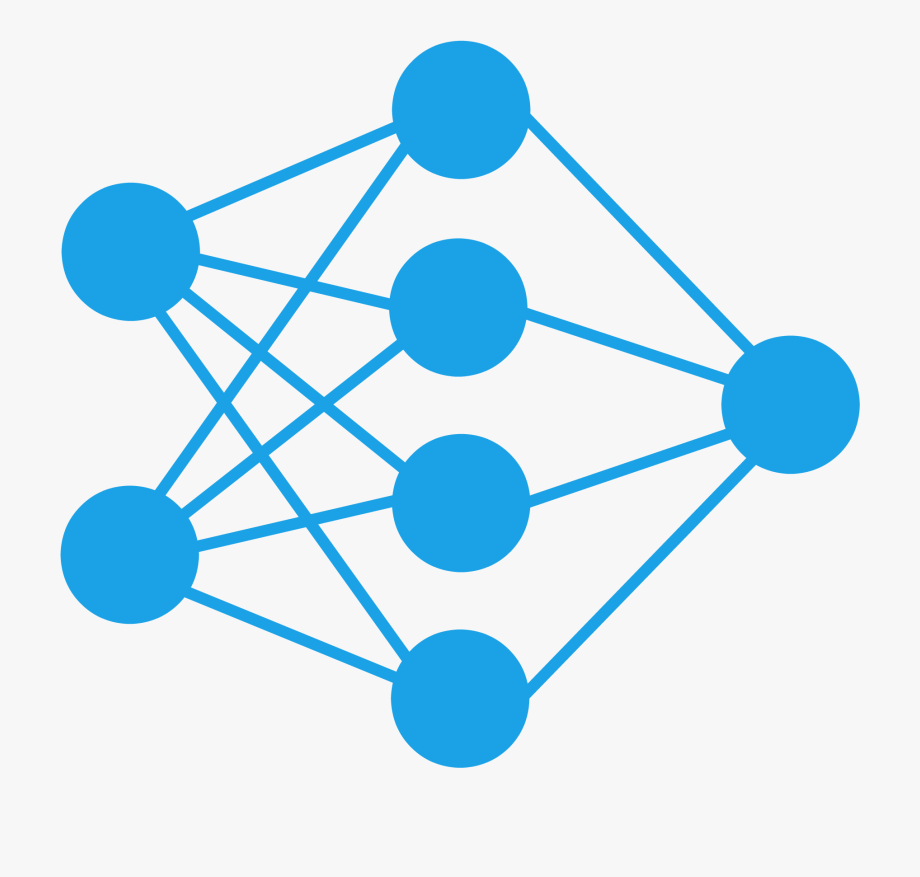
\includegraphics[width=0.5\linewidth,keepaspectratio]{./3_chapitre1/cover.png}}
 \node [inner sep=0pt](mypicture) at (0,0) {\phantom{\ig}};
 \clip[rounded corners=5mm] ($(mypicture.south west)+(\bord,\bord)$) rectangle ($(mypicture.north east)-(\bord,\bord)$);
 \node[inner sep=0pt](mypicture) at (0,0) {\ig};
\end{tikzpicture}
\end{center}

% Bullet points du début de chapitre
\begin{center}
\begin{colbox}{resume}
  \vspace{-2pt}
{\color{textresume}\small
\begin{itemize}[leftmargin=0in]\itemsep3pt
\item Nous avons entraîné un réseau de neurones convolutifs sur une base de données de près de \textbf{350 000} pour \textbf{61 classes} de coralligène et de substrat ~;
\item Le réseau final obtient une précision de \textbf{72.59 \% sur 61 classes}~;
\item La bonne calibration du réseau permet de faire une classification semi-automatique et de classer \textbf{67.48 \%} du jeu de données avec une précision de \textbf{85.65 \%}~;
\item En simplifiant la tâche de classification à 15 classes majeures, la précision atteint \textbf{84.47 \%}, soit une \underline{précision similaire à celle d'un expert taxonomiste}~;
\item Prédiction d'indicateurs de biodiversité et d'état de santé~:
\begin{itemize}
  \item \textbf{Shannon}~: bonne qualité prédictive (corrélation de Spearman 0.74)~;
  \item \textbf{CAI}~: qualité prédictive moyenne (corrélation de Spearman 0.61)~;
\end{itemize}
\end{itemize}
}
\vspace{-2pt}
%\end{fullminipage}
\end{colbox}
\end{center}

\clearpage

\noindent\textbf{Deep convolutional neural networks to monitor coralligenous reefs: operationalizing biodiversity and ecological assessment}

% Auteurs
%\noindent Guilhem Marre, Florian Holon, Sandra Luque, Pierre Boissery et Julie Deter

% NB sans indentation
\noindent\href{https://doi.org/10.1016/j.ecoinf.2020.101110}{\textit{Marre G, Holon F, Luque S, Boissery P and Deter J (2020) Deep convolutional neural networks to monitor coralligenous reefs: operationalizing biodiversity and ecological assessment. Ecological Informatics 59. doi: 10.1016/j.ecoinf.2020.101110}}

\medskip

\noindent\textbf{Abstract}
Monitoring the ecological status of natural habitats is crucial to the conservation process, as it enables the implementation of efficient conservation policies. Nowadays, it is increasingly possible to automate species identification, given the availability of very large image databases and state-of-the-art computational power which makes the training of automated machine learning-based classification models an increasingly viable tool for monitoring marine habitats. Coralligenous reefs are an underwater habitat of particular importance, found in the Mediterranean. This habitat is of a similar biocomplexity to coral reefs. They have been monitored in French waters since 2010 using manually annotated photo quadrats (RECOR monitoring network). Based on the large database of annotations accumulated therein, we have trained convolutional neural networks to automatically recognise coralligenous species using the data gathered from photo quadrats. Previous studies conducted on similar habitats performed well, but were only able to consider a limited number of classes, resulting in a very coarse description of these often-complex habitats. We therefore designed a custom network based on off-the-shelf architectures which is able to discriminate between 61 classes with 72.59 \% accuracy. Our results showed that confusion errors were for the most part taxonomically coherent, showing accuracy performances of 84.47 \% when the task was simplified to 15 major categories, thereby outperforming the human accuracy previously recorded in a similar study. In light of this, we built a semi-automated tool to reject unsure results and reduce error risk, for when a higher level of accuracy is required. Finally, we used our model to assess the biodiversity and ecological status of coralligenous reefs with the \gls{cai} and the Shannon Index. Our results showed that whilst the prediction of the CAI was only moderately accurate (pearson correlation between observed and predicted CAI = 0.61), the prediction of Shannon Index was more accurate (pearson correlation = 0.74). In conclusion, it will be argued that the approach outlined by this study offers a cost and time-effective tool for the analysis of coralligenous assemblages which is suitable for integration into a large-scale monitoring network of this habitat.

\noindent\textbf{Keywords}
Coralligenous reefs, Deep learning, Convolutional neural networks, Image classification, Species recognition, Monitoring

% Introduction
\section{Introduction}\label{chapitre1_1}
Coralligenous reefs represent unique calcareous formations of biogenic origin in the Mediterranean \citep{ballesteros_mediterranean_2006}; they are produced by the accumulation of encrusting algae and bioconstructor animals (polychaetes, bryozoans and gorgonians). Coralligenous reefs are similar to tropical coral reefs in terms of their richness, biomass, and production \citep{bianchi_biocostruzione_2001} and are considered the second richest marine habitat in the Mediterranean Sea \citep{boudouresque_marine_2004}. They are described as a special habitat with biodiversity interest by the European Habitats Directive (Habitats Directive 92/43/CEE). Like all marine ecosystems that are threatened on global scale by numerous anthropogenic pressures \citep{halpern_global_2008, hoekstra_confronting_2004}, coralligenous reefs are not exempt from the impacts of the Anthropocene \citep{mcgill_fifteen_2015} even if they are located at depths between 20 and 100 m below sea level. These coastal ecosystems are particularly sensitive to environmental changes as they are characterised by high levels of marine biodiversity \citep{halpern_global_2008} and are in contact with human population densities of about three times the average elsewhere \citep{small_global_2003}. They are severely affected by environmental pressures, most notably increasing sediment loads and deposition coming from human coastal activities and hydrodynamics alteration \citep{airoldi_effects_2003, ballesteros_mediterranean_2006}. This habitat desperately need to be monitored; “methods are urgently needed to assess prevailing patterns, evaluate impacts to which they [coralligenous outcrops] are subjected and provide baseline data to explore future trajectories of these high diversity assemblages” \citep{kipson_rapid_2011}.

Studying and monitoring the biodiversity of coralligenous reefs is limited by human physiological implications as it is physically demanding to spend a considerable amount of time at great depths underwater. Consequently, photo quadrats are commonly used in studies of this kind. This requires standardised photos to be taken by a diver in order for the coralligenous assemblages to be identified back on land \citep{deter_rapid_2012}. A taxonomist can measure a reef’s biodiversity (benthic species) and conservation status using indices such as the Coralligenous Assemblage Index (CAI) \citep{deter_preliminary_2012} and Shannon index \citep{magurran_measuring_2004}. This is however time-consuming, and requires well-trained taxonomists, as these reefs are home to over 1500 different species \citep{ballesteros_mediterranean_2006}. 

Since the mid-2000s, automated image classification has seen vast improvements, most notably in the development of deep Convolutional Neural Networks (CNNs). Most researchers now consider the task of image classification to have achieved its optimum potential (Rawat and Wang, 2017) in light of the outstanding performances of CNNs on well-known datasets such as ImageNet \citep{deng_imagenet:_2009}. Since CNNs first broke through in international image recognition challenges \citep{krizhevsky_imagenet_2012}, the networks have grown deeper and more efficient with various architectures \citep{he_deep_2016, huang_densely_2017, szegedy_going_2015}. Complications can nonetheless arise in applied cases such as species recognition. The variability of lighting conditions and intra-species morphological diversity renders underwater benthic species recognition particularly challenging \citep{beijbom_automated_2012}. Some studies have used machine learning algorithms for the identification of coral reefs species \citep{beijbom_automated_2012, marcos_classification_2005}). This habitat is similar to coralligenous reefs in terms of its richness and morphology \citep{bianchi_biocostruzione_2001}. In recent years, the application of state-of-the-art CNNs on coral datasets has achieved high classification accuracy, most notably when discriminating between coral and non-coral \citep{manderson_robotic_2017, williams_leveraging_2019}; they have achieved about 90 \% accuracy when identifying 10 different phylums \citep{king_comparison_2018}. Under human supervision, the use of a semi-automated framework has been shown to improve classification accuracy whilst remaining time and cost-effective \citep{beijbom_towards_2015, geifman_selective_2017}.

While no such framework has been tested on coralligenous reefs in particular, it should be noted that there is still room for improvement when applying CNNs to ecological data. At this point, the number of classes successfully recognised by CNNs is still relatively low, considering the wide variety of coralligenous species. Consequently, only a coarse level of analysis of broad taxa is possible. Discrimination among finer taxonomic levels is indeed a more complex task, as species and gender share a lot of visual characteristics and individual differences may be greater than inter-class variability. Taking into account the substantial cost of training such deep architectures, the networks used by most studies implementing CNNs for image classification were programmed with pre-trained weights which had been learnt on a different task \citep{king_comparison_2018, mahmood_deep_2017}, rather than training the networks from scratch. It has nevertheless been proven that, as the distance between the base task and the target task increases, the features’ transferability decreases \citep{yosinski_how_2014}. 

Our research therefore stems from the observation that, in previous work regarding benthic species recognition (i) the number of classes considered was limited when compared with the species richness generally encountered in coralligenous assemblages; (ii) the classes are mostly defined at a coarse taxonomical level (phylum, class, order); and (iii) the studies that achieved the highest classification accuracy when using CNNs used pre-trained networks that had been fine-tuned for the particular task at hand. We therefore aimed to expand upon the work done by previous studies on coralligenous reefs by building a fine-grained classifier, using state-of-the-art CNN architectures trained from scratch, in order to best address the task at hand.

\section{Related work}\label{chapitre1_2}
Over the last decade, the performance of supervised image classification algorithms has improved exponentially, owing to: the availability of very large labelled image databases such as ImageNet \citep{deng_imagenet:_2009}, developments in computational power, and the deepening of CNNs. These networks have been able to rapidly achieve state-of-the-art results in the most prestigious image recognition challenges \citep{russakovsky_imagenet_2015}. Since the challenge was first launched, research teams have sought new network architectures to improve classification performances. CNNs are now employed in a great variety of research fields including ecology, and are widely used for species recognition, notably the identification of coral species which they have performed excellently \citep{king_comparison_2018}.

To the best of our knowledge, no previous studies have attempted to automate the classification of coralligenous reef images. Coral reefs on the other hand have been extensively used as case studies for the development of automated visual assessment technologies, so that we may better monitor the biodiversity of these threatened ecosystems \citep{beijbom_automated_2012, beijbom_towards_2015, king_comparison_2018, mahmood_coral_2016, manderson_robotic_2017}. Coralligenous reefs are similarly as complex as coral reefs, and both are home to a multitude of different, intricate species \citep{bianchi_biocostruzione_2001}. We therefore used the performance of species recognition technology on coral reefs as a baseline for developing our own research techniques on coralligenous reefs.

\subsection{Annotator reliability}\label{chapitre1_2.1}
Underwater lightning conditions are subject to high variability due to the impaired light absorption by the water column, or ambient turbidity. Moreover, species identification is difficult because of the nuanced shapes and boundaries between species, and the high inter and intra-species morphological variability. These factors, combined with the variable quality of photo or video surveys \citep{manderson_robotic_2017}, leads to potential inconsistencies in the manual annotation of image datasets. 

To the best of our knowledge, very few studies assessed human error in the case of expert species identification, and only one studied this error in relation to the analysis of coral species \citep{beijbom_towards_2015}. Given the high similarity between coral and coralligenous reefs, and the lack of studies conducted on the latter habitat, we used the analysis of \citet{beijbom_towards_2015} as a baseline for expert annotation accuracy. Their dataset was composed of 800 images belonging to four different coral reefs across the Pacific Ocean, with 200 photos per site. Each image contained ten annotated random points with a resultant total of 2000 annotations per reef. The photographic survey was performed between 2005 and 2012 with a variety of different Digital Single Lens Reflex (DSLR) cameras, therefore the spatial resolution of the photos was variable and ranged between 12 and 81 pixels per mm2 for a size ranging from 6 to 10 Mpx. For each site, a local coral reef expert (named “host”) labelled the corresponding dataset with his own label-set. The four label-sets were mapped to a consensus set of 20 classes corresponding to miscellaneous non-living objects, whole phylum, and genders at the finer level of taxonomy. One to six years later, each site was presented for evaluation to six different experts: the “host” (the expert who established the ground truth annotation) and five “visitors” (coral experts with no prior knowledge of the study sites). These six experts labelled 2000 points per site according to the label set provided, resulting in 48000 annotations. The inter-annotator variability was assessed using Kappa statistic (Cohen, 1960). Results differed according to the considered functional group (coral, macroalgae, coralline algae or turf algae), and ranged from \(\kappa\) = 35.5 to 84.0 (i.e “minimal” to “strong” agreement between annotators). 

\subsection{CNNs for coral images classification}\label{chapitre1_2.2}
Previous attempts to use CNNs for coral images classification \citep{beijbom_improving_2016, king_comparison_2018, mahmood_deep_2017, mahmood_coral_2016}, outperformed other techniques based on hand-crafted features. In the event that there is a lack of data, or insufficient money to fund the cost of training state-of-the-art architectures, a CNN may first be trained using frozen, pre-trained weights on the convolutional layers, before the whole CNN is re-trained \citep{king_comparison_2018}. This procedure ensures that the imported weights are not significantly altered by the gradient descents. In their study, \citet{king_comparison_2018} used this method to benchmark different CNN architectures. They compared the accuracy on patch-based classification (bounding box around the annotated pixel) with VGG16, different implementations of Inception networks, and two ResNet networks (52 and 152 layers). The CNN that achieved the best classification accuracy in this ten-category coral classification task was the ResNet152, which attained 90.03 \% accuracy.

It has been shown that the patch size strongly influences classification performances \citep{beijbom_automated_2012}. The patch size may therefore be adjusted to optimise classification depending upon the size of the individual subjects and the particular location of the labelled pixel. A trade-off must be found, to include enough context while focusing on the information located at the centre of the patch \citep{beijbom_automated_2012} (see \autoref{figure1.1}). Local Spatial Pyramid Pooling (local-SPP) \citep{mahmood_coral_2016} improves feature extraction from point annotations, and makes the feature representation scale invariant. Patches of different scales are extracted and resized to fit the input size of a VGGnet (\(224 \times 244 pixels\)) and are then processed by the convolutional layers and the first fully connected layer in order to extract 4096-dimension feature vectors. All vectors obtained from the different patch sizes are max pooled to obtain a single feature vector which contains the highest values for the region considered. This approach enables a variety of scales to be processed, while max pooling renders the feature vector scale invariant.

%%%%%%%%%%%%%%%%%%%%%%%%%%%%%%%%%%%%%%%%%%%%%%%%%%%%%%%%%%%%%%%%%%%%
%%% Figure 1.1: Illustration of the patch size selection problem %%%
%%%%%%%%%%%%%%%%%%%%%%%%%%%%%%%%%%%%%%%%%%%%%%%%%%%%%%%%%%%%%%%%%%%%
\begin{figure}[H]
	\begin{center}
	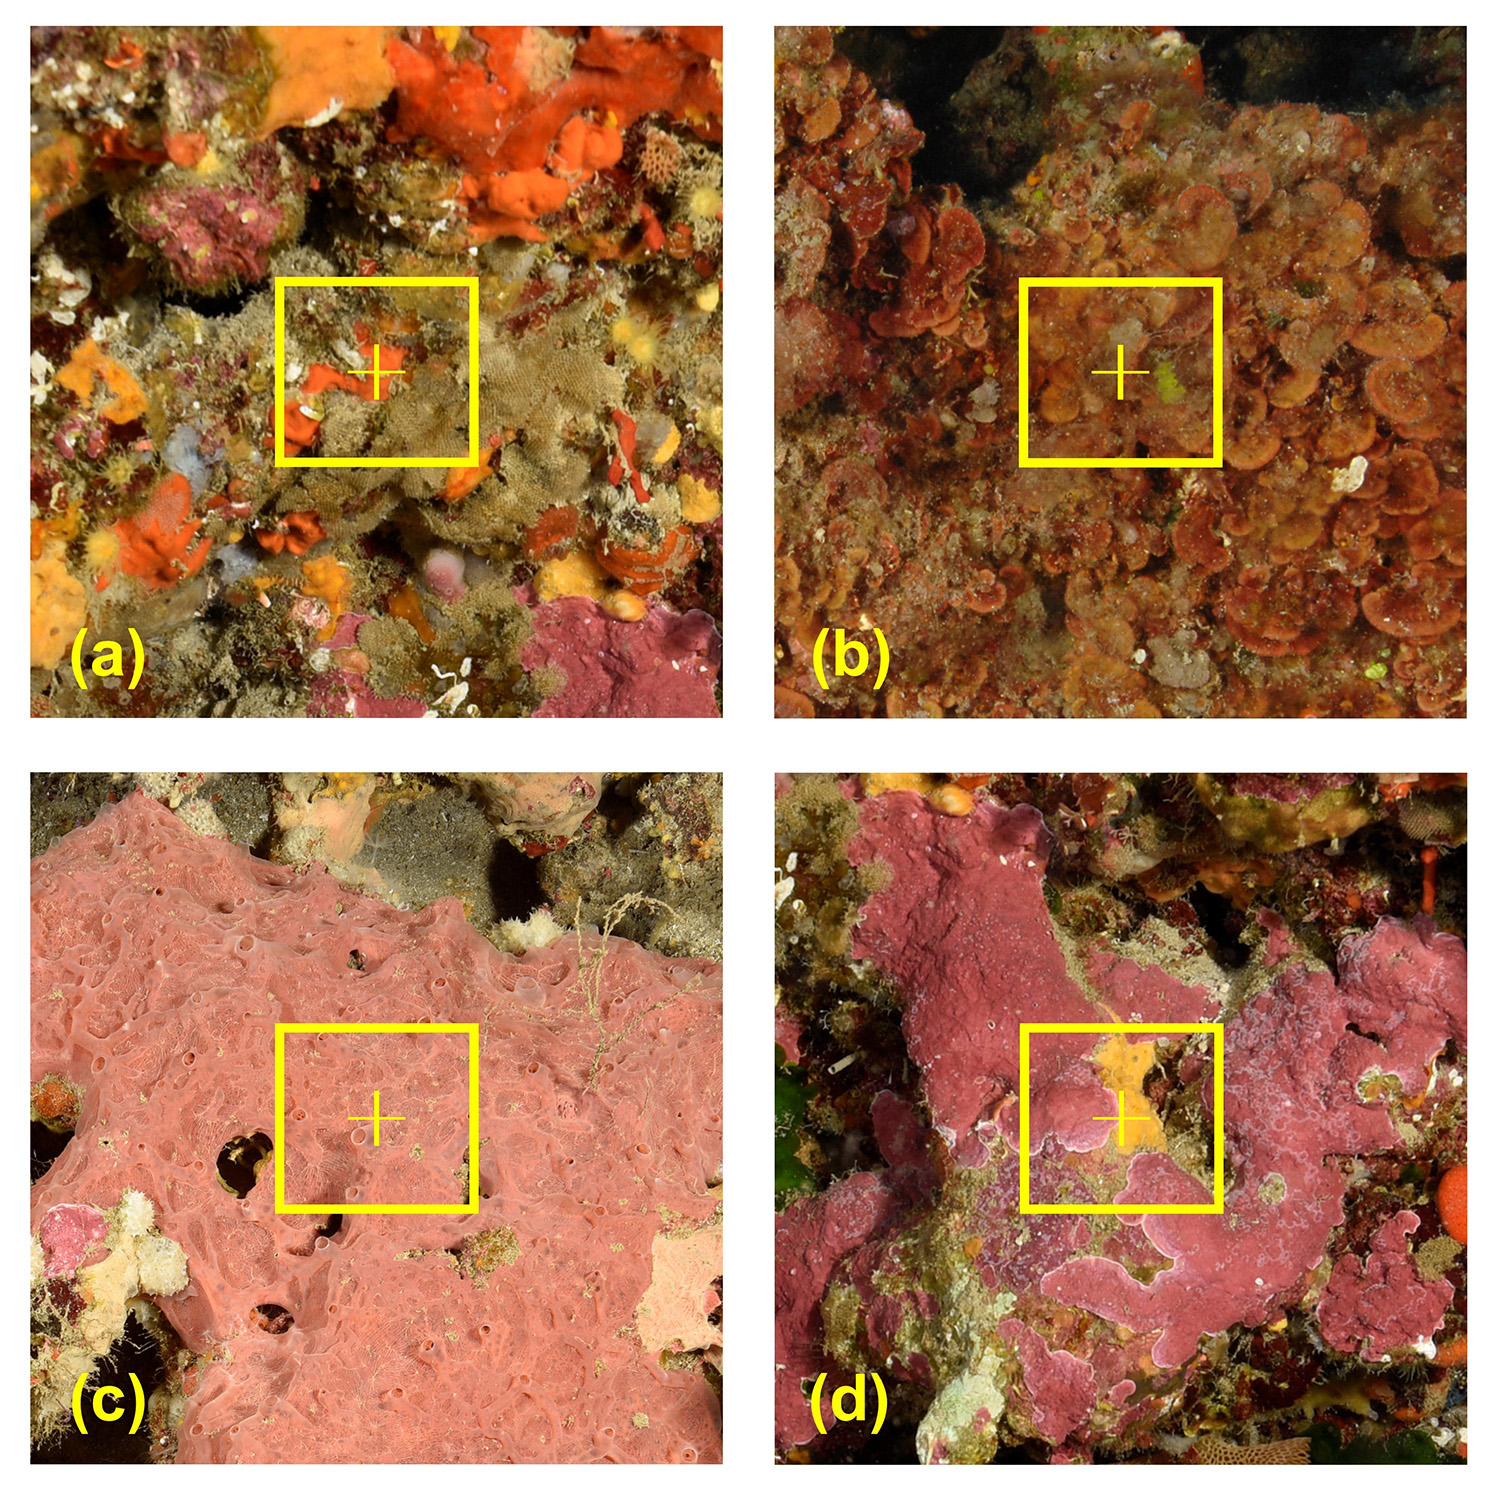
\includegraphics[width=0.6\linewidth,keepaspectratio]{./3_chapitre1/Figure1.1}
		\caption[Illustration of the patch size selection problem]{Illustration of the patch size selection problem. (a) the signal from the small sponge patch might be lost in its surroundings; (b) the patch might not capture the full extent of the larger textures; (c) extracted features would be more stable with a larger area; (d) point of interest on the edge between classes making any patch size problematic.}
	\label{figure1.1}
\end{center}
\end{figure}

\subsection{Automatic classification via deeply learned features}\label{chapitre1_2.3}
While neural networks excel at image classification, notably regarding famous challenges such as ImageNet, their performance can be curtailed in real-life classification problems, such as face recognition \citep{zhou_naive-deep_2015}, medicine \citep{de_fauw_clinically_2018} or species identification \\
\citep{mehdipour_ghazi_open-set_2016}. It should be noted that CNNs alone can struggle with datasets if some classes are under-represented; or if ground truth annotations are unreliable; or in the case of a fine-grained classification task, where there are intricate links between classes. Using CNNs in combination with other machine learning algorithms, such as: linear models, random forests, Logistic Regression (LR), and Support Vector Machines (SVMs) can improve classification performances \citep{gao_combining_2017, li_visual_2016}. \citet{li_visual_2016} used a random forest to process the feature activation map obtained from the ReLU of a layer of an AlexNet network concatenated with hand-crafted features, in order to improve saliency detection. In this instance the penultimate, fully connected layer provided the most discriminative features. Previous studies used SVMs trained with features from the convolutional layers of a CNN to improve classification accuracy \citep{gao_combining_2017, huang_large-scale_2006}. \citet{donahue_decaf:_2014}, who studied the influence of SVM and LR on classification performances using features extracted from different layers of a CNN \citep{donahue_decaf:_2014}, found that the 1st and 2nd fully connected layers improved the network the most, and that LR and SVM performed roughly equally as well. However, unlike SVMs, LR performs soft assignment and outputs probabilities making it naturally well-calibrated \citep{niculescu-mizil_predicting_2005}.

\section{Data}\label{chapitre1_3}

\subsection{Sampling procedure}\label{chapitre1_3.1}
Data were recorded over the period 2010---2018 during the RECOR monitoring network campaigns \citep{andromede-oceanologie_recor_2018}, from 198 sampling stations situated in 121 geographical locations along the French and Italian (Sardinia) Mediterranean coast. Each station was situated at a depth of between 17 and 90 m (see \autoref{figure1.2}), and a few of these locations included several sampling stations at various depths. 

%%%%%%%%%%%%%%%%%%%%%%%%%%%%%%%%%%%%%%%%%%%%%%%%%%%%%%%
%%% Figure 1.2: Localization of the 121 study sites %%%
%%%%%%%%%%%%%%%%%%%%%%%%%%%%%%%%%%%%%%%%%%%%%%%%%%%%%%%
\begin{figure}[H]
	\begin{center}
	%\captionsetup{width=.8\linewidth}
	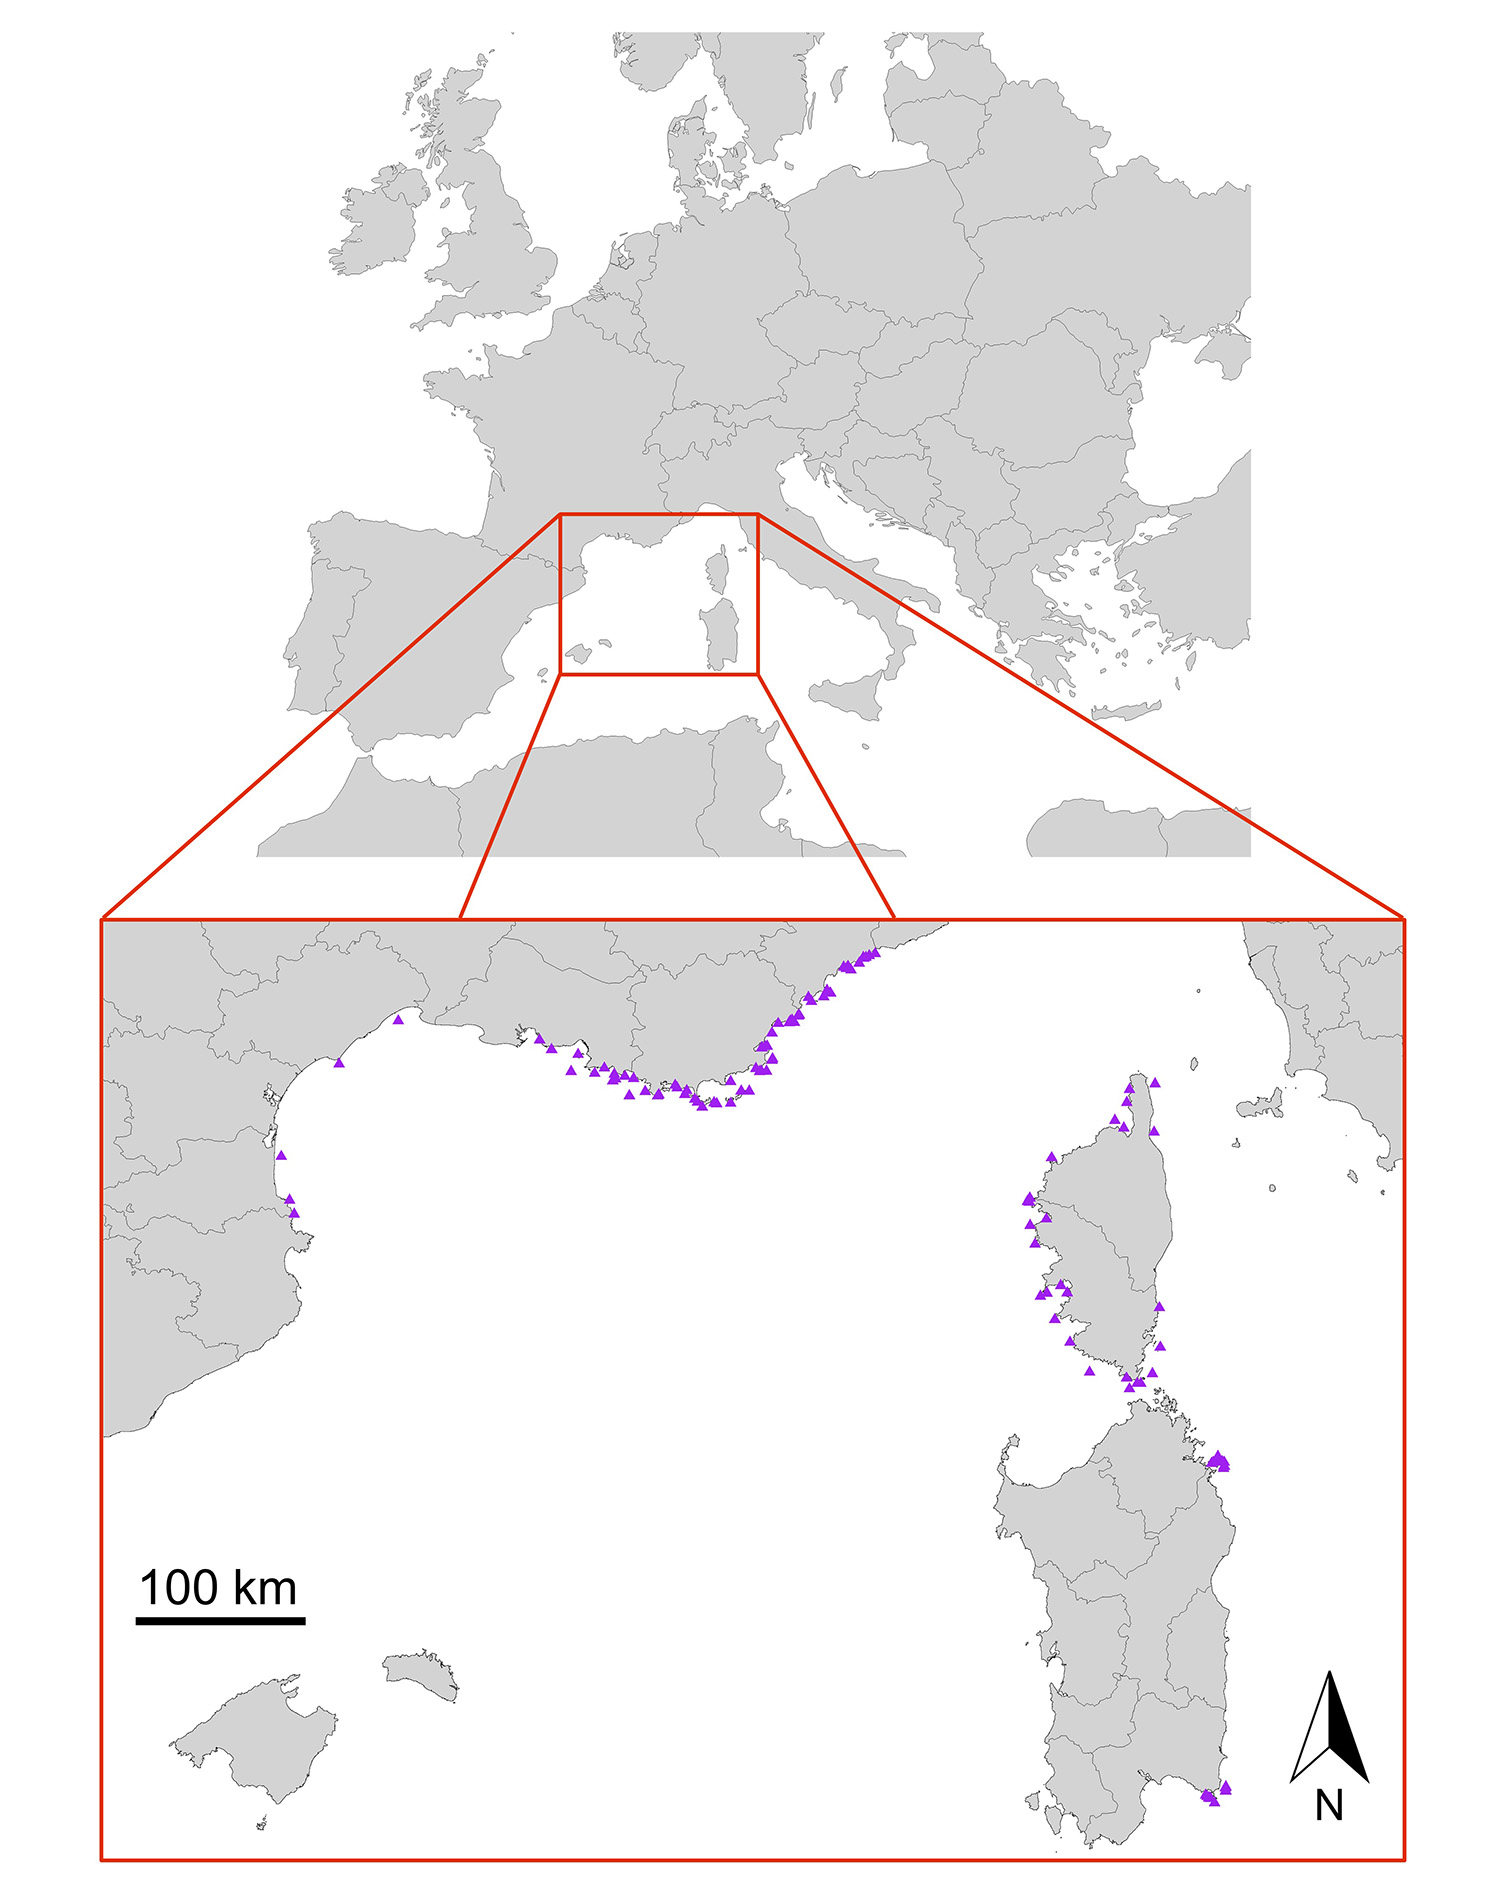
\includegraphics[width=0.8\linewidth,keepaspectratio]{./3_chapitre1/Figure1.2}
		\caption{Localization of the 121 study sites (South of France, Corsica and Sardinia).}
	\label{figure1.2}
\end{center}
\end{figure}

All photographic quadrats were acquired by one scuba diver, using a DSLR camera in a waterproof Seacam housing, fitted with two lateral strobes, fixed on a quadrat frame for standard acquisition (2500 cm² quadrat). Different cameras were used over the period 2010---2018: Nikon D2Xs, D3, D3S and D810. The resolutions ranged between 12.1 and 36.3 megapixels (Mpx), and had a focal length between 12 and 20 mm. Thirty quadrats were analysed per station, onto which 64 points were randomly projected (see \autoref{figure1.3}) and manually labelled using the Coral Point Count 4.1 \citep{cpce_coral_2011} software \citep{deter_rapid_2012}. 

%%%%%%%%%%%%%%%%%%%%%%%%%%%%%%%%%%%%%%%%%%%%%%%%%%%%%%%%%%%%%%%%
%%% Figure 1.3: Photographic quadrat of a coralligenous reef %%%
%%%%%%%%%%%%%%%%%%%%%%%%%%%%%%%%%%%%%%%%%%%%%%%%%%%%%%%%%%%%%%%%
\begin{figure}[H]
	\begin{center}
	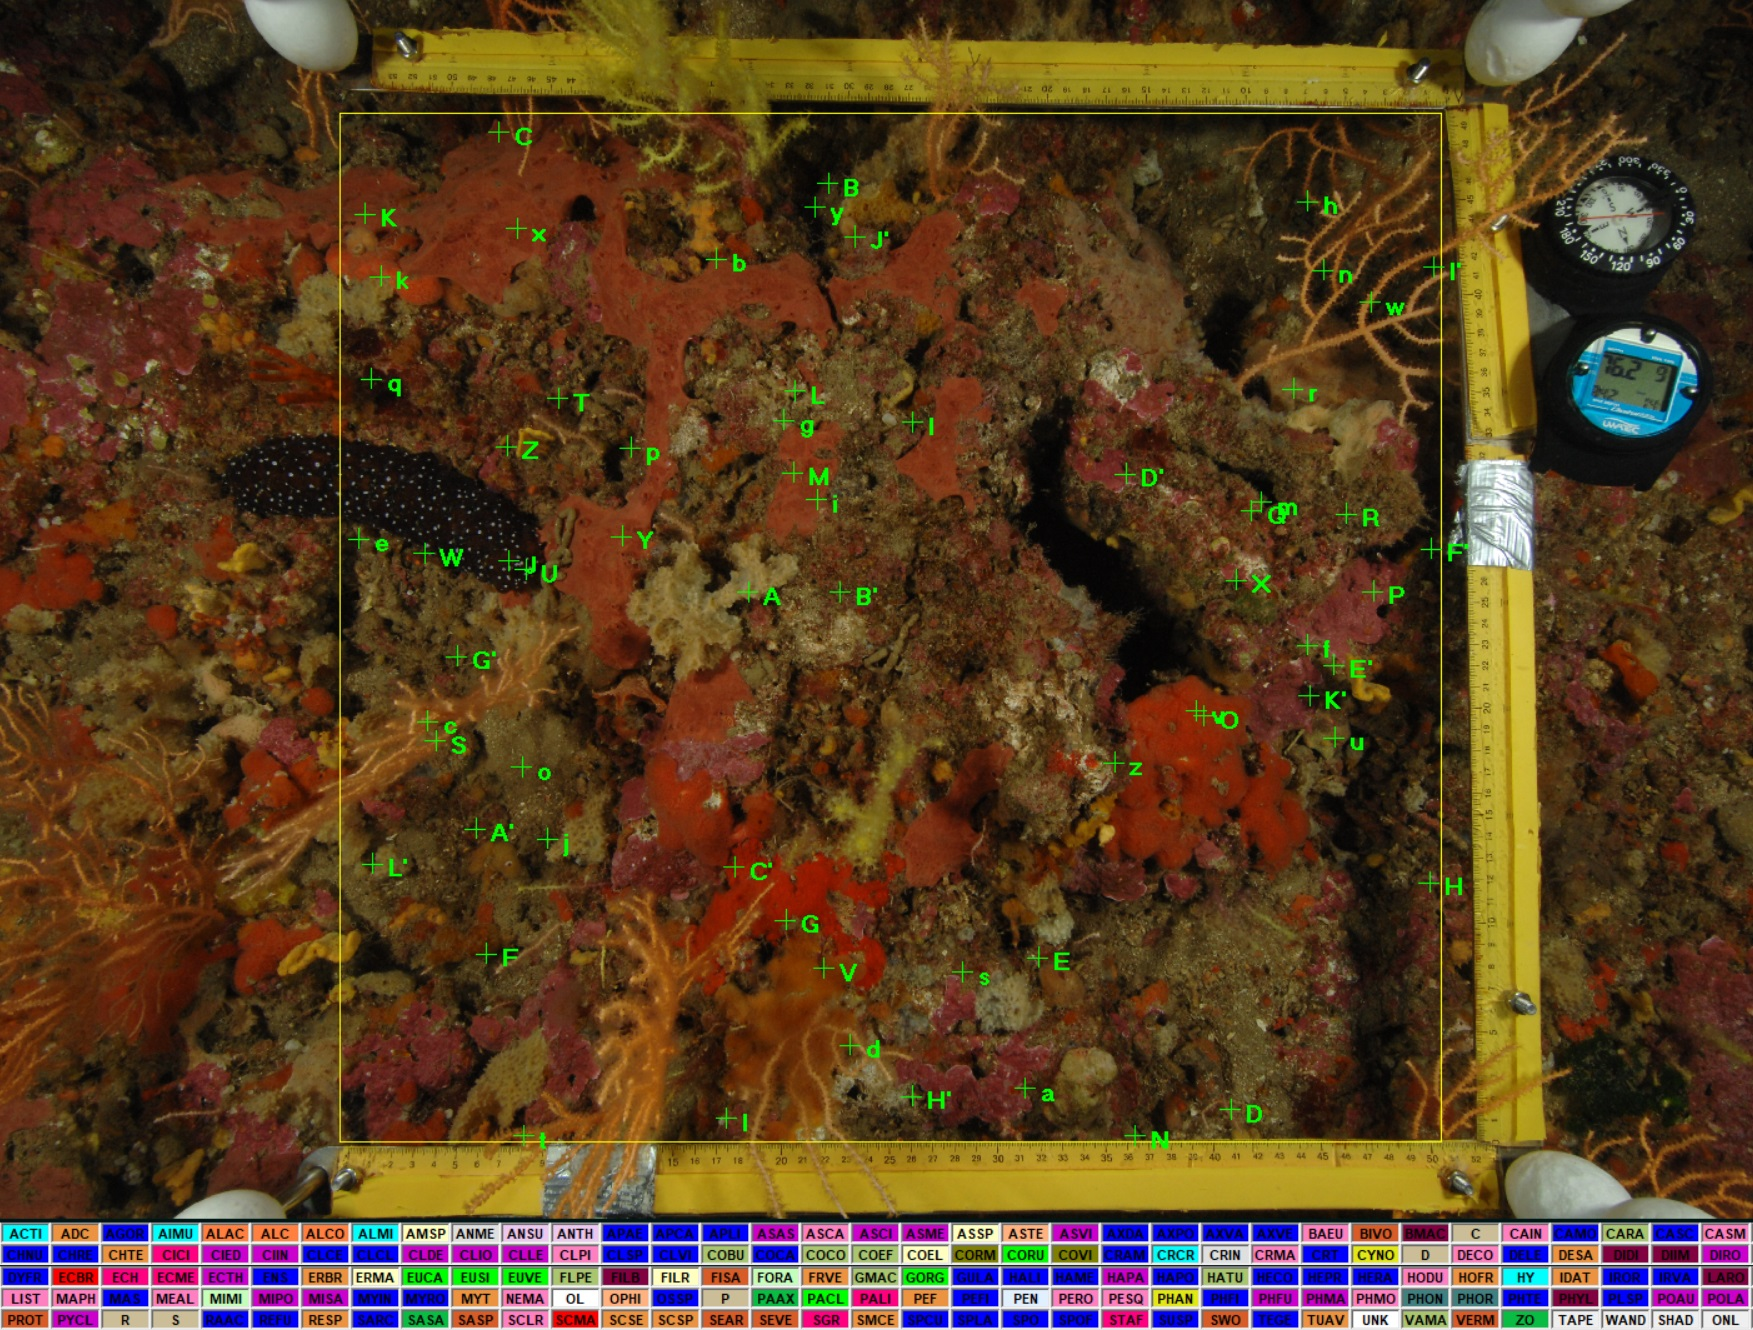
\includegraphics[width=0.8\linewidth,keepaspectratio]{./3_chapitre1/Figure1.3}
		\caption[Photographic quadrat of a coralligenous reef]{Photographic quadrat of a coralligenous reef. The green dots represent the 64 randomly projected points with CPCe software that are manually labelled.}
	\label{figure1.3}
\end{center}
\end{figure}

\subsection{Available dataset}\label{chapitre1_3.2}
The original dataset was composed of 668,160 annotations (made by the same taxonomic expert), sampled from 10,440 digital photographic quadrats. The database included 208 different classes and showed a high inter-class imbalance; the number of annotations per class ranged from 1 to over 100,000. All classes with less than approximately 500 instances were removed from the dataset, with the exception of “erected necrosis” (105 instances) because of the ecological importance to distinguish between erected and encrusted organisms, as they are not equally sensitive to anthropogenic pressures \citep{sartoretto_integrated_2017}. Undifferentiated sediment / substrate annotations from years 2010---2012 (labelled “sludge”, “pavement”, “rubble” and “sand” for years 2013---2018) were also removed from the dataset. Consequently, final dataset included 61 classes for a total of 349,370 annotations, and was then split into a training set of 282,940 annotations, a validation set of 34,963 annotations, and a test set of 31,467 annotations. The final dataset was somewhat more evenly balanced; each class was represented by 105 to 60,218 annotations.

\subsection{Biological links among classes }\label{chapitre1_3.3}
The biological relationships between classes describe a complex hierarchy at different taxonomic levels due to the impossibility / irrelevance of identifying all individuals up to species level from only visual analysis (see \autoref{figure1.4}; large circles represent the 61 classes subject to the classification task; small circles represent other classes that were not included) and intra-class variance is sometimes greater than inter-class variance (see \autoref{figure1.5}). Out of 61 classes, eight represent a coarse level of discrimination between major categories of living individuals, 31 classes may be identified at the species level (the finest level of discrimination apart from individuals), and the remaining categories were made up of 10 genders and 12 phylum or equivalent (broad categories of non-living objects). Many of these classes are closely related to each other and some classes of species belong to another gender class, themselves belonging to a major category class (see \autoref{figure1.4}).

%%%%%%%%%%%%%%%%%%%%%%%%%%%%%%%%%%%%%%%%%%%%
%%% Figure 1.4: Classes of coralligenous %%%
%%%%%%%%%%%%%%%%%%%%%%%%%%%%%%%%%%%%%%%%%%%%
\begin{figure}[H]
	\begin{center}
	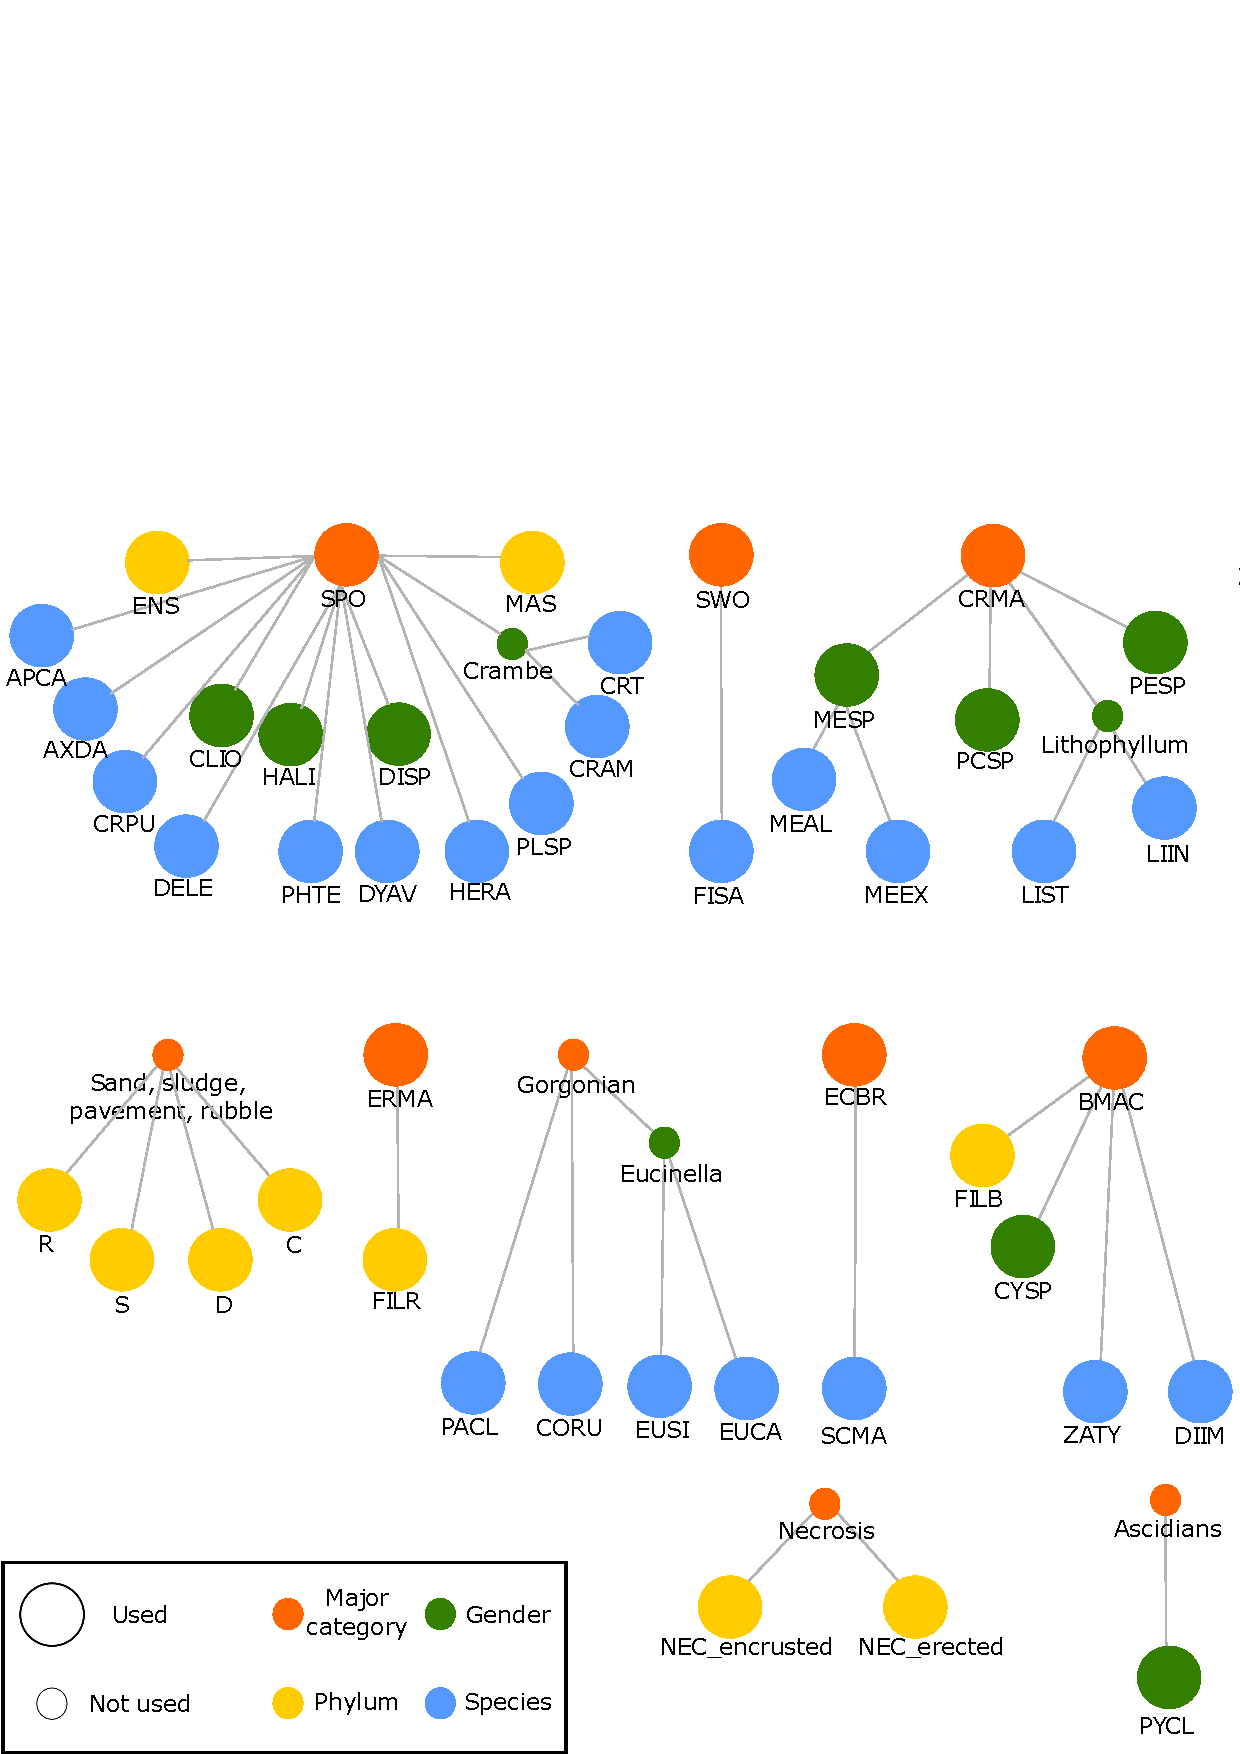
\includegraphics[width=\linewidth,keepaspectratio]{./3_chapitre1/Figure1.4}
		\caption[Classes of coralligenous taxa, hierarchically organised]{Classes of coralligenous taxa, hierarchically organised. Each network represents a major category (orange) linked to related phylums (yellow), genders (green) and species (blue). Smaller circles represent categories not subject to the original classification task and are written out in words. ADC = \textit{Adeonella calveti}; APCA = \textit{Aplysina cavernicola}; AXDA = \textit{Axinella damicornis}; BMAC = \textit{Brown macroalgae}; C = Crevice; CELL = \textit{Cellaria sp.}; CLIO = \textit{Cliona sp.}; CORU = \textit{Corallium rubrum}; CRAM = \textit{Crambe crambe}; CRMA = Encrusting red macroalgae; CRPU = \textit{Crella pulvinar}; CRSP = \textit{Crisia sp.}; CRT = \textit{Crambe tailliezi}; CYSP = \textit{Cystoseira sp.}; D = Sand; DELE = \textit{Dendroxea lenis}; DIIM = \textit{Dictyota implexa}; DISP = \textit{Dictyonella sp.}; DYAV = \textit{Dysidea avara}; ECBR = Encrusting bryozoan; ENS = Non identified encrusting sponge; ERBR = Erected bryozoan; ERMA = Erected red macroalgae; EUCA = \textit{Eunicella cavolini}; EUSI = \textit{Eunicella singularis}; FILB = Filamentous brown algae; FILG = Filamentous green algae; FILR = Filamentous red algae; FISA = \textit{Filograna} or \textit{Salmacina sp.}; FLPE = \textit{Flabellia petiolate}; GMAC = Green macroalgae; HALI = \textit{Haliclona sp.}; HATU = \textit{Halimeda tuna}; HERA = \textit{Hexadella racovitzai}; HY = Hydrozoa; LEPR = \textit{Leptopsammia pruvoti}; LIIN = \textit{Lithophyllum incrustans}; LIST = \textit{Lithophyllum stictaeforme}; MAS = Non identified massive sponge; MEAL = \textit{Mesophyllum alternans}; MEEX = \textit{Mesophyllum expansum}; MESP = \textit{Mesophyllum sp.}; MYT = \textit{Myriapora truncate}; NEC$\_$encrusted = Encrusted necrosis; NEC$\_$erected = Erected necrosis; PAAX = \textit{Parazoanthus axinellae}; PACL = \textit{Paramuricea clavata}; PACR = \textit{Palmophyllum crissum}; PCSP = Encrusting \textit{Peyssonnelia sp.}; PEF = \textit{Pentapora fascialis}; PESP = Erected \textit{Peyssonnelia sp.}; PHTE = \textit{Phorbas tenacior}; PLSP = \textit{Pleraplysilla spinifera}; PYCL = \textit{Pycnoclavella sp.}; R = Rubble; S = Sludge; SCMA = \textit{Schizomavella mamillata}; SPO = Sponges; SWO = Sedentary worms; VAMA = \textit{Valonia macrophysa}; ZATY = \textit{Zanardinia typus}.}
	\label{figure1.4}
\end{center}
\end{figure}

For instance, Mesophyllum alternans (MEAL) and Mesophyllum expansum (MEEX) are different species belonging to the same gender Mesophyllum sp (MESP), and Mesophyllum sp belongs to the major category Encrusting red macroalgae (CRMA). These classes also share a lot of visual characteristics, and it is the task of the algorithm to find the features common to one particular class which are not shared by specific subcategories. This requires an expert knowledge and is qualified as a fine-grained classification task \citep{akata_evaluation_2015}.

%%%%%%%%%%%%%%%%%%%%%%%%%%%%%%%%%%%%%%%%%%%%%%%%%%
%%% Figure 1.5: intra and inter-class variance %%%
%%%%%%%%%%%%%%%%%%%%%%%%%%%%%%%%%%%%%%%%%%%%%%%%%%
\begin{figure}[H]
	\begin{center}
	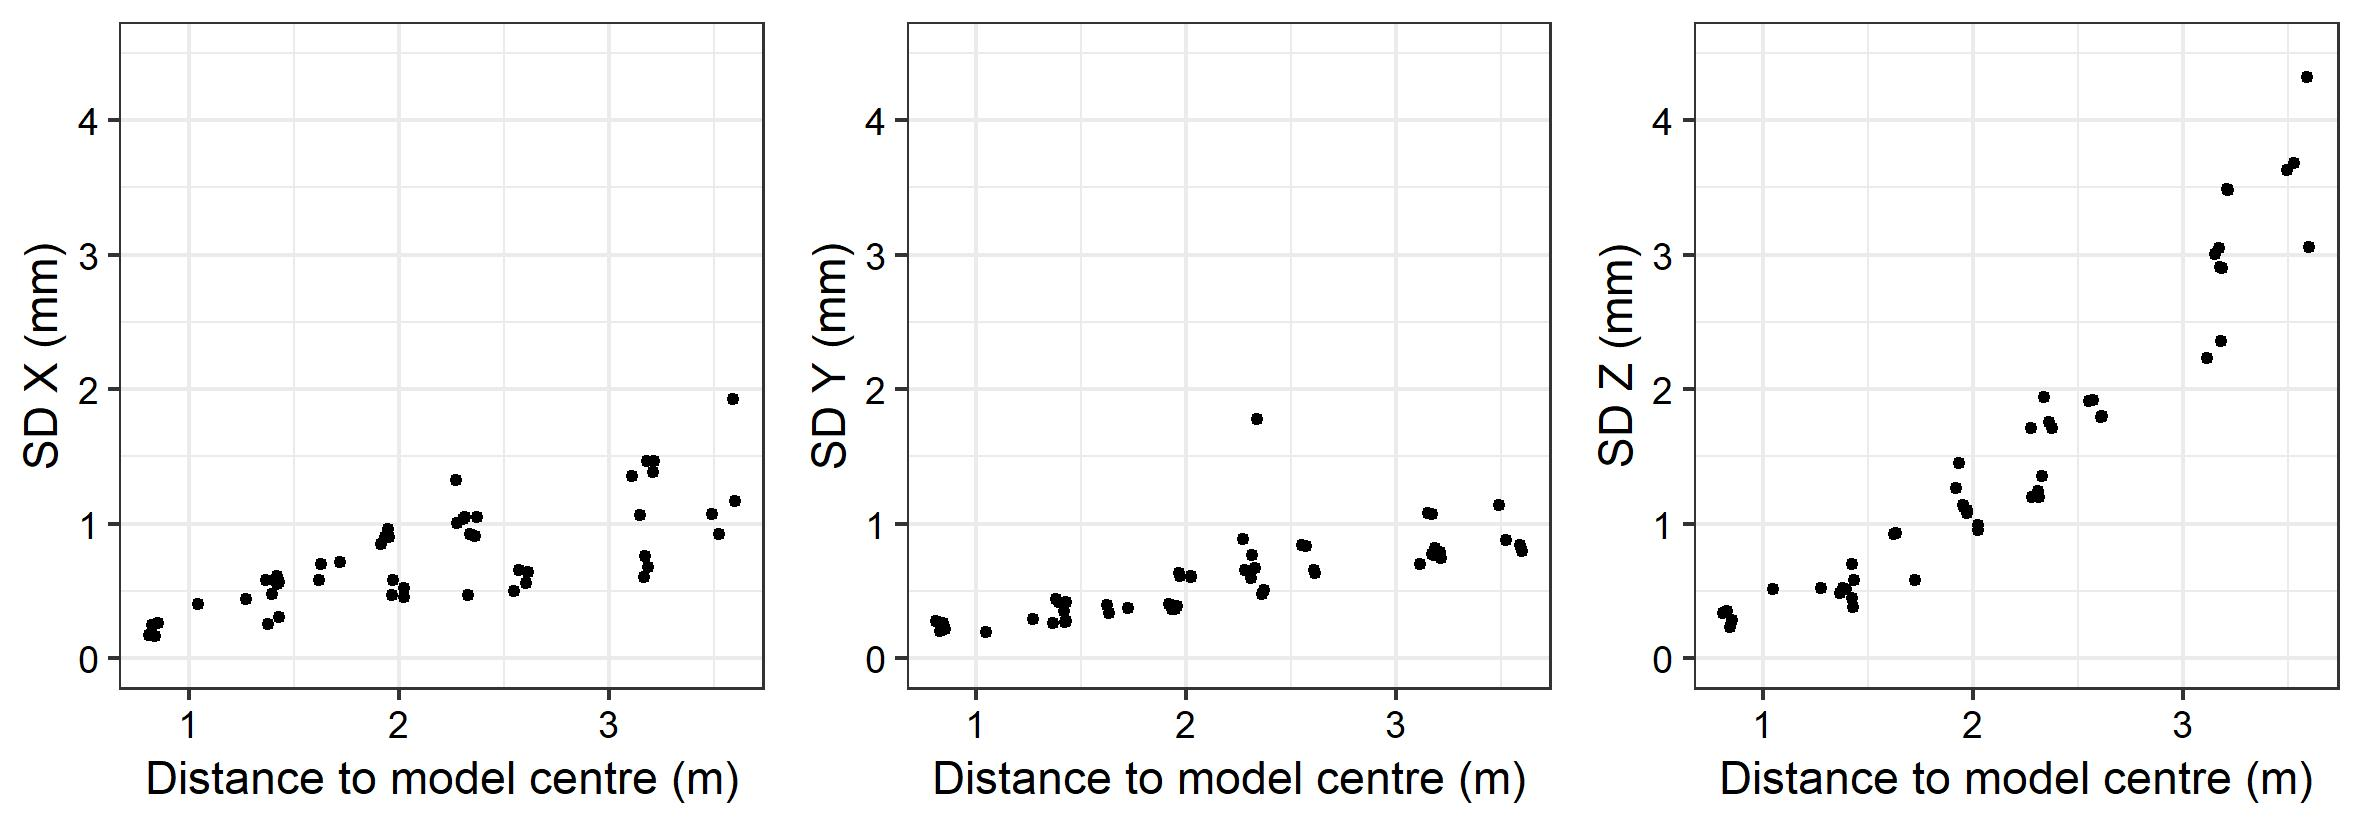
\includegraphics[width=0.8\linewidth,keepaspectratio]{./3_chapitre1/Figure1.5}
		\caption[Illustration of intra and inter-class variance]{Illustration of intra and inter-class variance. MEAL = Mesophyllum alternans; MEEX = Mesophyllum expansum; MESP = Mesophyllum sp.; CRMA = Encrusting red macroalgae.}
	\label{figure1.5}
\end{center}
\end{figure}

\section{Methodology}\label{chapitre1_4}

This study sought to design and train an algorithm based on deep CNN architectures, in order to identify a selection of coralligenous species or their broader taxonomical group, and to assess the biodiversity and ecological status of coralligenous reefs. We designed a custom methodology, drawing on state-of-the-art architectures and a large database of annotated photographic quadrats. More specifically, we performed the following analysis :

\begin{enumerate}
\item Assess human annotation error on a similar problem in order to establish a baseline performance;
\item Train simple CNNs on different patch sizes and build an ensemble network in order to improve performances with multi-scale prediction;
\item Train a LR on deeply learned features from intermediate layers to improve performances and calibrate the ensemble network;
\item Build a semi-automated tool based on the calibrated ensemble network, allowing to classify a dataset with a required minimum error risk;
\item Reduce the classification level of detail by grouping classes to higher taxonomical degrees (56 genders and 15 major categories), to build a customizable tool able to classify at different levels of details with corresponding accuracies.
\end{enumerate}

\subsection{Assessment of annotator reliability}\label{chapitre1_4.1}
We used the data from \citet{beijbom_towards_2015} (see \autoref{chapitre1_2.1}) to assess human annotator accuracy using F1-score (see section 5.2.1). For each point, the ground truth was defined as the first identification by the “host” expert. These results will be used to discuss our CNN classification performances.

\subsection{Ensemble network for multi-scale prediction}\label{chapitre1_4.2}
Different studies showed that in a patch-based classification context, multiple scales classification improved the final performances of the classifier \citep{beijbom_automated_2012, mahmood_coral_2016}. Indeed, many cases can challenge a patch-based classifier (small vs large individuals, point located on the edge between two classes…), and the integration of analyses made at different scales can help build a more robust and discriminative classifier. Therefore, we trained an ensemble of ResNet18s on four patch sizes (see \autoref{figure1.6}): \(224 \times 224\), the standard input sizes for most CNNs, \(128 \times 128\), \(96 \times 96\), and \(64 \times 64\) pixels. However, our methodology slightly differs from earlier works in two main aspects. Firstly, \citet{mahmood_coral_2016} resized the extracted patches to fix input dimensions as they used a pre-trained network. Conversely, we trained ResNet18s from scratch and consequently, input size was able to correspond to the size of the extracted patches. This avoids information loss which comes as a consequence of upscaling of small patches. Secondly, instead of implementing a max pooling set on the last convolutional layer \citep{mahmood_coral_2016}, our ensemble network uses the four outputs from the Global Average Pooling (GAP) layers, following the last convolutional block of the trained ResNet18. This ensures that more information is preserved and can be processed by a Multi-Layer Perceptron (MLP) and the concatenation results in a 2048 features vector. Our MLP was made up of three fully connected layers, of sizes 512 (fc512), 256 (fc256) and 61; the first two layers used ReLU activation, and the final layer a softmax, for classification.


\subsection{Logistic regression with deeply learned features}\label{chapitre1_4.3}
We trained LR models with different inputs, from the features learned by the deep learning model (output of the concatenation layer feeding the MLP; see Figure 6), to the more processed logits of the softmax layer:

\begin{itemize}
    \item Features from the concatenation of GAP outputs; 
    \item Features from the first layer of the MLP (fc512);
    \item Features from the second layer of the MLP (fc256);
    \item Logits of the softmax layer;
    \item Concatenation of the features of fc256 and the logits (see Figure 6). 
    
\end{itemize}

%%%%%%%%%%%%%%%%%%%%%%%%%%%%%%%%%%%%%%%%%%%%%%%%%%%%%
%%% Figure 1.6: Structure of the ensemble network %%%
%%%%%%%%%%%%%%%%%%%%%%%%%%%%%%%%%%%%%%%%%%%%%%%%%%%%%
\begin{figure}[H]
	\begin{center}
	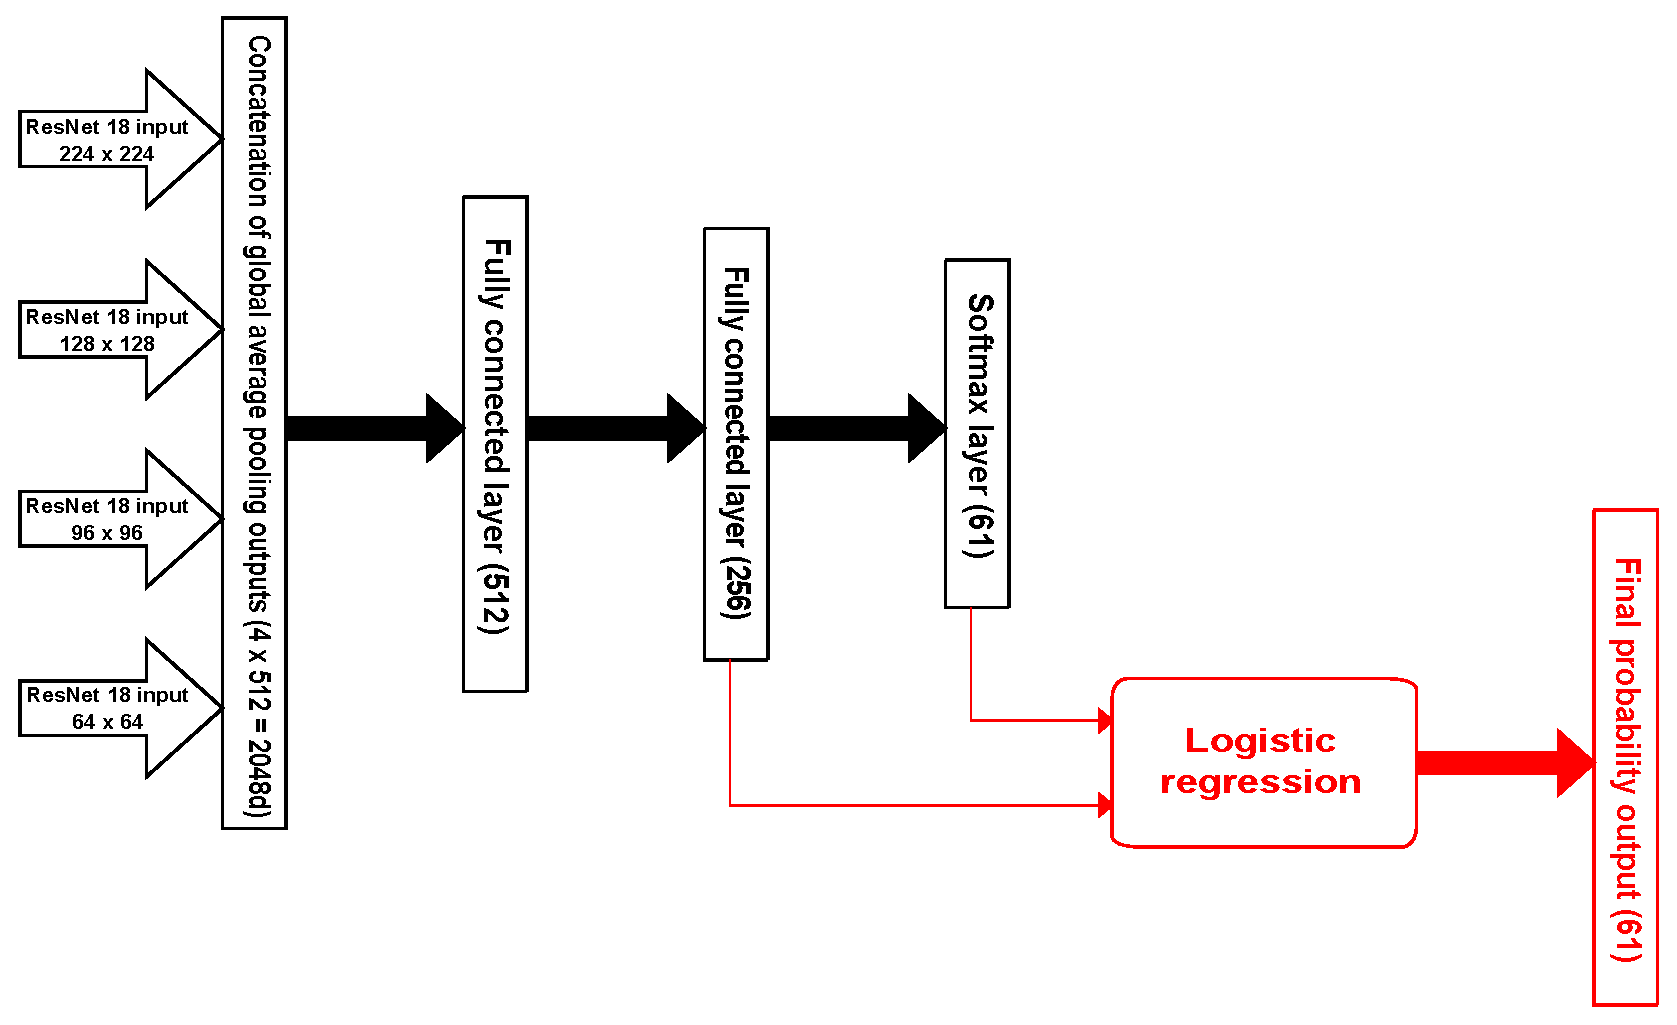
\includegraphics[width=\linewidth,keepaspectratio]{./3_chapitre1/Figure1.6}
		\caption[Structure of the ensemble network]{Structure of the ensemble network without (black) and with (red) machine learning prediction on deeply learned features (outputs of the two last layers of the MLP are concatenated and passed as input to a logistic regression). Features from global average pooling layer of four ResNet18s are fed to a MLP made of three fully connected layers of size: 512 and 256 with ReLU activation, and 61 with softmax for classification.}
	\label{figure1.6}
\end{center}
\end{figure}

\subsection{Semi-automated framework with selective classification}\label{chapitre1_4.4}
Selective classification, also called “reject option” \citep{herbei_classification_2006}, is a technique used to optimise classification performance. By training a classifier to decide whether or not a prediction is reliable, this technique reduces the error rate at the cost of a decrease in the classification rate, since the algorithm rejects certain samples which can later be manually labelled by an expert. This has been empirically investigated previously, in the case of image classification of marine habitats \citep{beijbom_automated_2012, beijbom_towards_2015}. Thresholding is a simple and fast method for mitigating a lack of performances in the classification task, in the event that the accuracy of human annotations in the dataset is lacking. Within a more theoretical framework, the use of selective classification with neural networks has previously been studied to find the best possible rejection rule \citep{geifman_selective_2017}. They called this risk-coverage approach “Selection with Guaranteed Risk” (SGR). For a given desired risk (i.e misclassification rate), the SGR maximises classification coverage while keeping the risk below the limit. 

Implementation of selective classification requires a good calibration of the network, i.e. the network should output a probability score equivalent to the empirical accuracy; for an output score of 0.8 for example, the network should predict the right class in 80 \% of the cases. However, a recent study showed that deep neural networks are not always well calibrated, and they tend to output over-confident prediction scores \citep{guo_calibration_2017}. Hyperparameters, such as depth, batch normalization, and weight decay, have been shown to influence calibration. Scaling the logits passed to the softmax function can also help calibrate the network.


\subsection{Categories merging: from coarse-to-fine biodiversity assessment}\label{chapitre1_4.5}
In order to provide different levels of analysis ranging from coarse to fine, and to enhance classification performances, we analysed the classification results at different taxonomic levels by grouping classes by gender or major category after classification with the 61-class network. As seen above, the relations between classes describe a complex and interconnected schema. Degrading the level of detail for the classification task was therefore expected to increase classification accuracy, as the different class levels were set according to a taxonomic hierarchy between original classes that share common visual characteristics. Level 1 corresponds to the original classification task (61 classes), level 2 corresponds to a classification at the gender level (54 classes; see Figure 4), and level 3 corresponds to the major category (15 classes). Furthermore, level 3 grouping describes a reduced number of classes which allowed us to have insight into class-wise performances and distribution.

\section{Experimental settings}\label{chapitre1_5}

\subsection{Training procedure}\label{chapitre1_5.1}
It has been previously established that on a similar case which involved patch-based coral classification, the ResNet152 architecture performed best \citep{king_comparison_2018}. However, this architecture is very deep and considers tens of millions of parameters. Consequently, we experimented on different, shallower CNNs which were modelled on this architecture (ResNet18 and ResNet50). Unlike many previous studies which used transfer learning \citep{king_comparison_2018, mahmood_coral_2016, mahmood_deep_2017}, we trained our CNNs from scratch. Different ResNet18s were trained with batch normalization and ReLU activation taking place before the convolution layer, as this has been proven to improve generalization \citep{he_identity_2016}. We trained these CNNs using Adam optimiser, with a learning rate of $10^{-3}$ and other parameters set to their defaults, in accordance with the original study \citep{kingma_adam:_2014}. Data was fed iteratively in batches of 512, for patches of dimensions \(64 \times 64\), \(96 \times 96\) and \(128 \times 128\) pixels. Batches of 200 were used for patch size \(224 \times 224\) due to computational limitations. A ResNet50 was also trained under the same conditions, with patch size \(128 \times 128\) and batch size 128, once again due to computational limitations. In order to better compare the networks, a ResNet18 was also trained with same conditions as the ResNet50. The ensemble network was built on four ResNet18s (see \autoref{figure1.6}) which were independently trained on the four patch sizes. The ensemble was then fine-tuned: we used a batch size of 128, froze the weights from the ResNet18s, and used the same optimiser and parameters as mentioned above. Data augmentation on all patches was performed for all trained networks, in order to compensate for the high class imbalance and allow a better generalization. We applied random rotations between 0 and 180 degrees, brightness scaling between 0.4 and 1.6, and horizontal / vertical flipping to all patches on the fly as data was fed to the networks. Trainings lasted at least 100 epochs and were stopped when validation accuracy did not improve for 25 epochs.

A ResNet152 was used as the baseline for classification performance. This network was initially programmed using pre-trained weights lifted from the ImageNet challenge. The top fully-connected layer was replaced with a layer using ReLU activation, followed by a dropout layer and a softmax layer, with outputs corresponding to the number of classes (here 61). Firstly, the top layer was trained alone; using features extracted from the convolutional layers, a Stochastic Gradient Descent (SGD) with a learning rate of $10^{-3}$, and weight decay rate set to $5\times10^{-4}$. The whole network was then trained with SGD; learning rate$10^{-4}$ and weight decay $10^{-6}$. Patches of \(224 \times 224\) were fed in batches of 16. Training was performed over 50 epochs until loss on the validation set stopped decreasing.

The deeply learned features and the different layer outputs of the training, validation, and test sets were extracted in advance. LRs were trained and optimised using the grid search tool implemented in scikit-learn\footnote{Scikit-learn v0.20.2} on the validation set.

SGR was applied at risk levels ranging from 5 to 30 \% and resultant thresholds. Coverages and bounds for the coverage were assessed together with top-5 accuracy on the unclassified part of the dataset. SGR was trained on the validation set and applied to the training and test set with the aforementioned risk levels to assess the corresponding coverages.

All architectures were implemented in Python 3.6 using the Keras\footnote{Keras v 2.2.4} library and Tensorflow\footnote{Tensorflow v 1.12.0} backend. All training and testing processes were performed on a Windows 10 workstation with 64 bits OS, 128 Gb RAM, \(2 \times\)NVidia GeForce GTX 1080 Ti 11 Gb memory and 12 cores CPU 2.9 GHz.

\subsection{Evaluation metrics}\label{chapitre1_5.2}

\subsubsection{Classification performances}\label{chapitre1_5.2.1}

The performances of the networks were assessed with the precision, recall and F1-score. At training, validation and testing time; precision, recall and F1-score were calculated as follows:

\begin{equation}
\text{F1-score}=2\times\frac{\text{Precision}\times\text{Recall}}{\text{Precision}+\text{Recall}}
\label{eq1.1}
\end{equation}

With:

\begin{equation}
\text{Precision}=\frac{\text{True Positive}}{\text{True Positive}+\text{False Positive}}
\label{eq1.2}
\end{equation}

\begin{equation}
\text{Recall}=\frac{\text{True Positive}}{\text{True Positive}+\text{False Negative}}
\label{eq1.3}
\end{equation}

F1 ranges from 0 to 1, 1 being a perfect classifier.

The three metrics were computed at both micro and macro levels. Micro-F1, precision, and recall computed the statistics across all classes, given their distribution on the whole dataset, while macro statistics placed equal weight on all classes, meaning that class-wise differences in performance more greatly impacted the scores. This rendered micro-recall equivalent to the overall top-1 accuracy of the models (these two terms will be used interchangeably).

\subsubsection{Calibration of the networks}\label{chapitre1_5.2.2}

After training, network calibration was evaluated on the validation set for the best ResNet18, the baseline ResNet152, and the ensemble network with and without LR. Predictions were grouped in M bins of same size for the computation of accuracy according to the following equation \citep{guo_calibration_2017}:

\begin{equation}
	acc(B_m)=\frac{1}{|B_m|}\sum_{i\in B_m}\textbf{1}(\hat{y}_i=y_i)
	\label{eq1.4}
\end{equation}

Where $B_m$ is the set of indices of the instances composing bin $m$, $\hat{y}_i$ the predicted class of instance $i$ and $y_i$ its true class. Average confidence for $B_m$ is then given by :

\begin{equation}
conf(B_m)=\frac{1}{|B_m|}\sum_{i\in B_m}\hat{p}_i
\label{eq1.5}
\end{equation}

With $\hat{p}_i$ the outputted probability corresponding to the class $\hat{y}_i$. On top of the diagrams, Estimated Calibration Error (ECE) was calculated for the models considered with the following equation.

\begin{equation}
\text{ECE}=\sum_{m=1}^{M}\frac{|B_m|}{n}|acc(B_m)-conf(B_m)|
\label{eq1.6}
\end{equation}

With $n$ the total number of samples in the dataset.


\subsubsection{Coralligenous ecological status and biodiversity assessment}\label{chapitre1_5.2.3}
Coralligenous health is typically assessed using the Coralligenous Assemblage Index (CAI) \citep{deter_preliminary_2012}. This is based on the prevalence of bryozoans, major builders and sludge in an assemblage. The CAI is calculated as follows:

\begin{equation}
\text{CAI\textsubscript{i}}=\frac{1}{3}\times(\frac{1-sludge_i}{1-\min_{i}sludge_i}+\frac{majbuilders_i}{\max_{i}majbuilders_i}+\frac{bryozoans_i}{\max_{i}bryozoans_i})
\label{eq1.7}
\end{equation}

With \textit{sludge\textsubscript{i}}, \textit{majbuilders\textsubscript{i}} and \textit{bryozoans\textsubscript{i}}, the covering percentage of sludge, major builders (13 classes out of the 61) and bryozoans (8 classes out of the 61) respectively. Minimum and maximum values of these percentages are calculated over all study sites. CAI is classically measured on 30 quadrats, 64 points per quadrat, for a total of 1,920 annotated points.

Biodiversity indices are numerous. This includes simpler indices, such as species richness which refers to the number of observed species, and more integrated indices which take abundance into account in order to attribute more or less weight to common or rare species \citep{magurran_measuring_2004}. One commonly used index is the Shannon index:

\begin{equation}
	S_j=-\sum_{i}p_{ij} log(p_{ij})
	\label{eq1.8}
\end{equation}

With \textit{p\textsubscript{ij}} the prevalence of species \textit{i} among site \textit{j}.

Both indices were modelled by randomly selecting 10,000 sets of 1,920 instances from the test set of 31,467 instances). For each set of 1,920, proportions of sludge / bryozoans / major builders, CAI and Shannon index were calculated on the ground truth and the automatic labels. Pearson correlations were used to analyse the fit between true and modelled indices.

\section{Results}\label{chapitre1_6}

\subsection{Human error}\label{chapitre1_6.1}
The assessment of human annotator reliability on the dataset presented in section 2.1 showed variable performances across the expert panel (see \autoref{table1.1}). All metrics were significantly higher for the hosts (who performed the ground truth annotation) than visitors, and micro-F1 was higher than macro-F1 for both the hosts and visitors.


%%%%%%%%%%%%%%%%%%%%%%%%%%%%%%%
%%% Table 1.1: Human error  %%%
%%%%%%%%%%%%%%%%%%%%%%%%%%%%%%%
\begin{table}[htbp]
  \centering
  \normalsize
 % \raggedright
  \caption[Classification accuracy of hosts (n = 4) and visitors (n = 20) on the Moorea dataset]{Classification accuracy of hosts (n = 4) and visitors (n = 20) on the Moorea dataset (Beijbom et al., 2012). \textit{Values are given in mean percentage ± standard deviation.}}
  \label{table1.1}
    \begin{tabular}{*{4}{c}}
        \toprule
        \textbf{Subject} & \textbf{Macro-F1} & \textbf{Top-1 accuracy} & \textbf{Micro-F1} \\ \midrule
        hosts            & 74.86 ± 3.63      & 79.21 ± 2.35            & 80.32 ± 2.32      \\
        visitors         & 59.4 ± 4.15       & 64.98 ± 6.31            & 68.31 ± 4.64      \\ \bottomrule
    \end{tabular}
\end{table}

\subsection{CNN performances}\label{chapitre1_6.2}

\subsubsection{Simple CNNs and ensemble network}\label{chapitre1_6.2.1}
All validation performances consistently increased with the patch size up to 224 × 224, which achieved 65.94 micro-F1 (see \autoref{table1.2}). As for training curves, the gap between patch size performances tended to decrease quickly. It is worth emphasizing that macro-F1 (with all classes weighted equally) was consistently lower than micro-F1 (all classes weighted according to their proportion in the dataset).

%%%%%%%%%%%%%%%%%%%%%%%%%%%%%%%%%%%%%%%%%
%%% Table 1.2: Performances ResNet18  %%%
%%%%%%%%%%%%%%%%%%%%%%%%%%%%%%%%%%%%%%%%%
\begin{table}[htbp]
  \centering
  \normalsize
  %\raggedright
  \caption[Performances of the ResNet18 on the validation and test sets for different input sizes]{Performances of the ResNet18 on the validation and test sets for different input sizes (patch size). In bold the best value for each metric.}
  \label{table1.2}
  %\scalebox{0.95}[0.95]{
    \begin{tabular}{*{2}{c}|*{3}{c}|*{3}{c}}
        \toprule
        \multicolumn{2}{c}{\textbf{}}             & \multicolumn{3}{c}{\textbf{Validation set}}                     & \multicolumn{3}{c}{\textbf{Test set}}                           \\ 
        \midrule
        \textbf{Patch Size} & \makecell{\textbf{Batch} \\ \textbf{size}} & \textbf{Macro-F1} & \makecell{\textbf{Top-1} \\ \textbf{accuracy}} & \textbf{Micro-F1} & \textbf{Macro-F1} & \makecell{\textbf{Top-1} \\ \textbf{accuracy}} & \textbf{Micro-F1} \\ \midrule
        64 × 64             & 512                 & 40.29             & 54.43                   & 55.07             & 46.50             & 60.64                   & 60.17             \\
        96 × 96             & 512                 & 51.21             & 63.97                   & 63.73             & 51.75             & 63.82                   & 63.57             \\
        128 × 128           & 512                 & 54.28             & 65.99                   & 65.85             & 54.08             & 65.77                   & 65.54             \\
        224 × 224           & 200                 & 54.93             & 66.70                   & 66.44             & 53.93             & 66.30                   & 65.94             \\ \bottomrule
    \end{tabular}
    %}
\end{table}

The ResNet18 and ResNet50 trained with the same hyperparameters  (see \autoref{table1.3}, ResNet50---128 and ResNet18---128) performed roughly equally on validation and test sets, with ResNet18-128 achieving a micro-F1 of 63.44 and ResNet50 63.89 on the test set. However, an epoch for the ResNet50 took about three times longer than ResNet18. The ResNet50 did not outperform the previously trained ResNet18 with patch size 128 and batch size 512 (see \autoref{table1.2}). The deeper architecture of the ResNet50 made it impossible to train with a batch size of 512.

%%%%%%%%%%%%%%%%%%%%%%%%%%%%%%%%%%%%%%%%%%%%%%%%%%%%%
%%% Table 1.3: Performances of different ResNet   %%%
%%%%%%%%%%%%%%%%%%%%%%%%%%%%%%%%%%%%%%%%%%%%%%%%%%%%%
\begin{table}[htbp]
  \centering
  \normalsize
 % \raggedright
  \caption[Performances of different ResNet architectures on validation and test sets]{Performances of different ResNet architectures on validation and test sets. ResNetX---Y is written so that X indicates the network’s depth and Y the input size. In bold the best value for each metric.}
  \label{table1.3}
    \begin{tabular}{*{2}{c}|*{3}{c}|*{3}{c}}
        \toprule
        \multicolumn{2}{c}{\textbf{}}                      & \multicolumn{3}{c}{\textbf{Validation set}}                     & \multicolumn{3}{c}{\textbf{Test set}}                           \\ \midrule
        \textbf{Network} & \makecell{\textbf{Batch} \\ \textbf{size}} & \textbf{Macro-F1} & \makecell{\textbf{Top-1} \\ \textbf{accuracy}} & \textbf{Micro-F1} & \textbf{Macro-F1} & \makecell{\textbf{Top-1} \\ \textbf{accuracy}} & \textbf{Micro-F1} \\
        \midrule
        ResNet152---224                & 16                  & 37.45             & 62.38                   & 60.46             & 38.26             & 61.71                   & 60.09             \\
        ResNet50---128                 & 128                 & 52.04             & 64.07                   & 63.85             & 52.27             & 64.35                   & 63.89             \\
        ResNet18---128                 & 128                 & 51.40             & 63.90                   & 63.88             & 51.62             & 63.60                   & 63.44             \\
        ResNet18---224                 & 200                 & 54.93             & 66.70                   & 66.44             & 53.93             & 66.30                   & 65.94             \\
        Ensemble                     & 128                 & \textbf{60.56}    & \textbf{70.60}          & \textbf{70.35}    & \textbf{60.38}    & \textbf{70.54}          & \textbf{70.37}    \\ \bottomrule
    \end{tabular}
\end{table}

The ensemble network performed better than any previous CNN on validation and test sets (70.35 and 70.37 micro-F1, respectively), and outperformed both the best, single ResNet18 (65.94, see \autoref{table1.2}) and the baseline ResNet152 (60.09, see \autoref{table1.3}). The latter performed worse than any other network considered here for all metrics, with macro-F1 (37.45 and 38.26 on validation and test sets, respectively) lower than micro scores (micro-F1 of 60.46 and 60.09). With the sole exception of CNN for patch size 64 \(\times\) 64, validation and test performances were very similar for all trained models, and macro metrics were consistently lower than micro metrics.

\subsubsection{Ensemble network with logistic regression}\label{chapitre1_6.2.2}
LRs were trained using l2 penalty and multinomial loss, with the following parameters defined with grid search on the validation set: C = 0.01 and saga solver\footnote{Grid search : C = \{10-4 ; 10\textsuperscript{-3} ; 10\textsuperscript{-2} ; 10\textsuperscript{-1} ;1 ;10 ;100\} ; solver = \{sag ; saga ; lbfgs\}}. Results were compared with each other and with the ensemble alone (see \autoref{table1.4}).

%%%%%%%%%%%%%%%%%%%%%%%%%%%%%%%%%%%%%%%%%%%%%%%%%%%%%%%%
%%% Table 1.4: Performances of logistic regression   %%%
%%%%%%%%%%%%%%%%%%%%%%%%%%%%%%%%%%%%%%%%%%%%%%%%%%%%%%%%
\begin{table}[htbp]
    \centering
      \caption[Performances of logistic regression applied to different layers of the ensemble network, on validation and test sets]{Performances of logistic regression applied to different layers of the ensemble network, on validation and test sets. None: ensemble alone, logits: features of the last layer before softmax, fc256: features from the penultimate layer; fc512: features from the first layer of the Multi-Layer Perceptron (MLP); GAP: features from the concatenation of global average pooling before the MLP. In bold the best value for each metric.}
      \label{table1.4}
    \begin{tabular}{*{1}{c}|*{3}{c}|*{3}{c}}
    	\toprule
    	\textbf{} & \multicolumn{3}{c}{\textbf{Validation set}} & \multicolumn{3}{c}{\textbf{Testing set}}\\
    	\midrule
    	\textbf{Features} & \textbf{Macro-F1} & \textbf{Top-1 accuracy} & \textbf{Micro-F1} & \textbf{Macro-F1} & \textbf{Top-1 accuracy} & \textbf{Micro-F1}\\
    	\midrule%[0.05cm] % épaisseur du trait
    	None & 60.56 & 70.60 & 70.35 & 60.38 & 70.54 & 70.37\\
    	logits & 61.93 & 72.23 & 71.81 & 61.69 & 71.91 & 71.50\\
    	fc256 & \textbf{63.92} & 72.62 & 72.28 & 62,69 & 72.41 & 72.02\\
    	fc512 & 16.31 & 55.09 & 53.23 & 8.55 & 44.12 & 42.37\\
    	GAP & 10.12 & 46.67 & 45.19 & 6.70 & 38.64 & 37.31\\
    	combined & 63.74 & \textbf{72.69} & \textbf{72.32} & \textbf{63.91} & \textbf{72.59} & \textbf{72.20}\\
    	\bottomrule
    \end{tabular}
\end{table}

The LR on the logits and features from the penultimate layer (fc256) resulted in an improvement in both macro and micro metrics scores, compared with the ensemble network alone (see “None”, \autoref{table1.4}). On the test set, micro-F1 increased from 70.37 to 71.50 using logits, and 72.02 using the penultimate layer, while macro-F1 increased from 60.38 to 61.69 and 62.69 respectively. The use of both layers’ features (see “fc256 + logits”, \autoref{table1.4}) resulted in a marginal improvement (63.91 for macro-F1 and 72.20 for micro-F1 on the test set). Using features from the first layer of the MLP (fc512), or the concatenation of global average pooling outputs, resulted in consistent degradation of all metrics on the validation set, and results were even worse for the test set. Using the best model, out of the 61 classes, 11 showed an accuracy >80 \% (\textit{“Aplysina cavernicola”}, “Crevice”, \textit{“Corallium rubrum”}, \textit{“Crambe tailliezi”}, \textit{“Eunicella cavolini”}, \textit{“Hexadella racovitzai”}, \textit{“Leptopsammia pruvoti”}, \textit{“Mesophyllum alternans”}, \textit{“Parazoanthus axinellae”}, \textit{“Paramuricea clavata”}, \textit{“Erected Peyssonnelia sp.”}) and 12 had an accuracy comprised between 70 \% and 80 \% (“Sand”, \textit{“Eunicella singularis”}, “Filamentous green algae”, “Filamentous red algae”, \textit{”Flabellia petiolata”}, \textit{“Haliclona sp.”}, \textit{“Halimeda tuna”}, \textit{“Palmophyllum crassum”}, \textit{“Encrusting Peyssonnelia sp.”}, \textit{“Pentapora fascialis”}, \textit{“Phorbas tenacior”}, \textit{“Pleraplysilla spinifera”}).

\subsection{Post-processing}\label{chapitre1_6.3}

\subsubsection{Semi-automated classification}\label{chapitre1_6.3.1}
Reliability diagrams –which plot confidence against accuracy – were plotted for the baseline ResNet152, the best ResNet18, and the ensemble network with and without LR (see \autoref{figure1.7}). The red line shows a theoretical, perfect calibration (y = x).

%%%%%%%%%%%%%%%%%%%%%%%%%%%%%%%%%%%%%%%%%%%%%%%%%%%%%%%%%%%%%%%%%%
%%% Figure 1.7: Reliability diagrams of the different networks %%%
%%%%%%%%%%%%%%%%%%%%%%%%%%%%%%%%%%%%%%%%%%%%%%%%%%%%%%%%%%%%%%%%%%
\begin{figure}[H]
	\begin{center}
	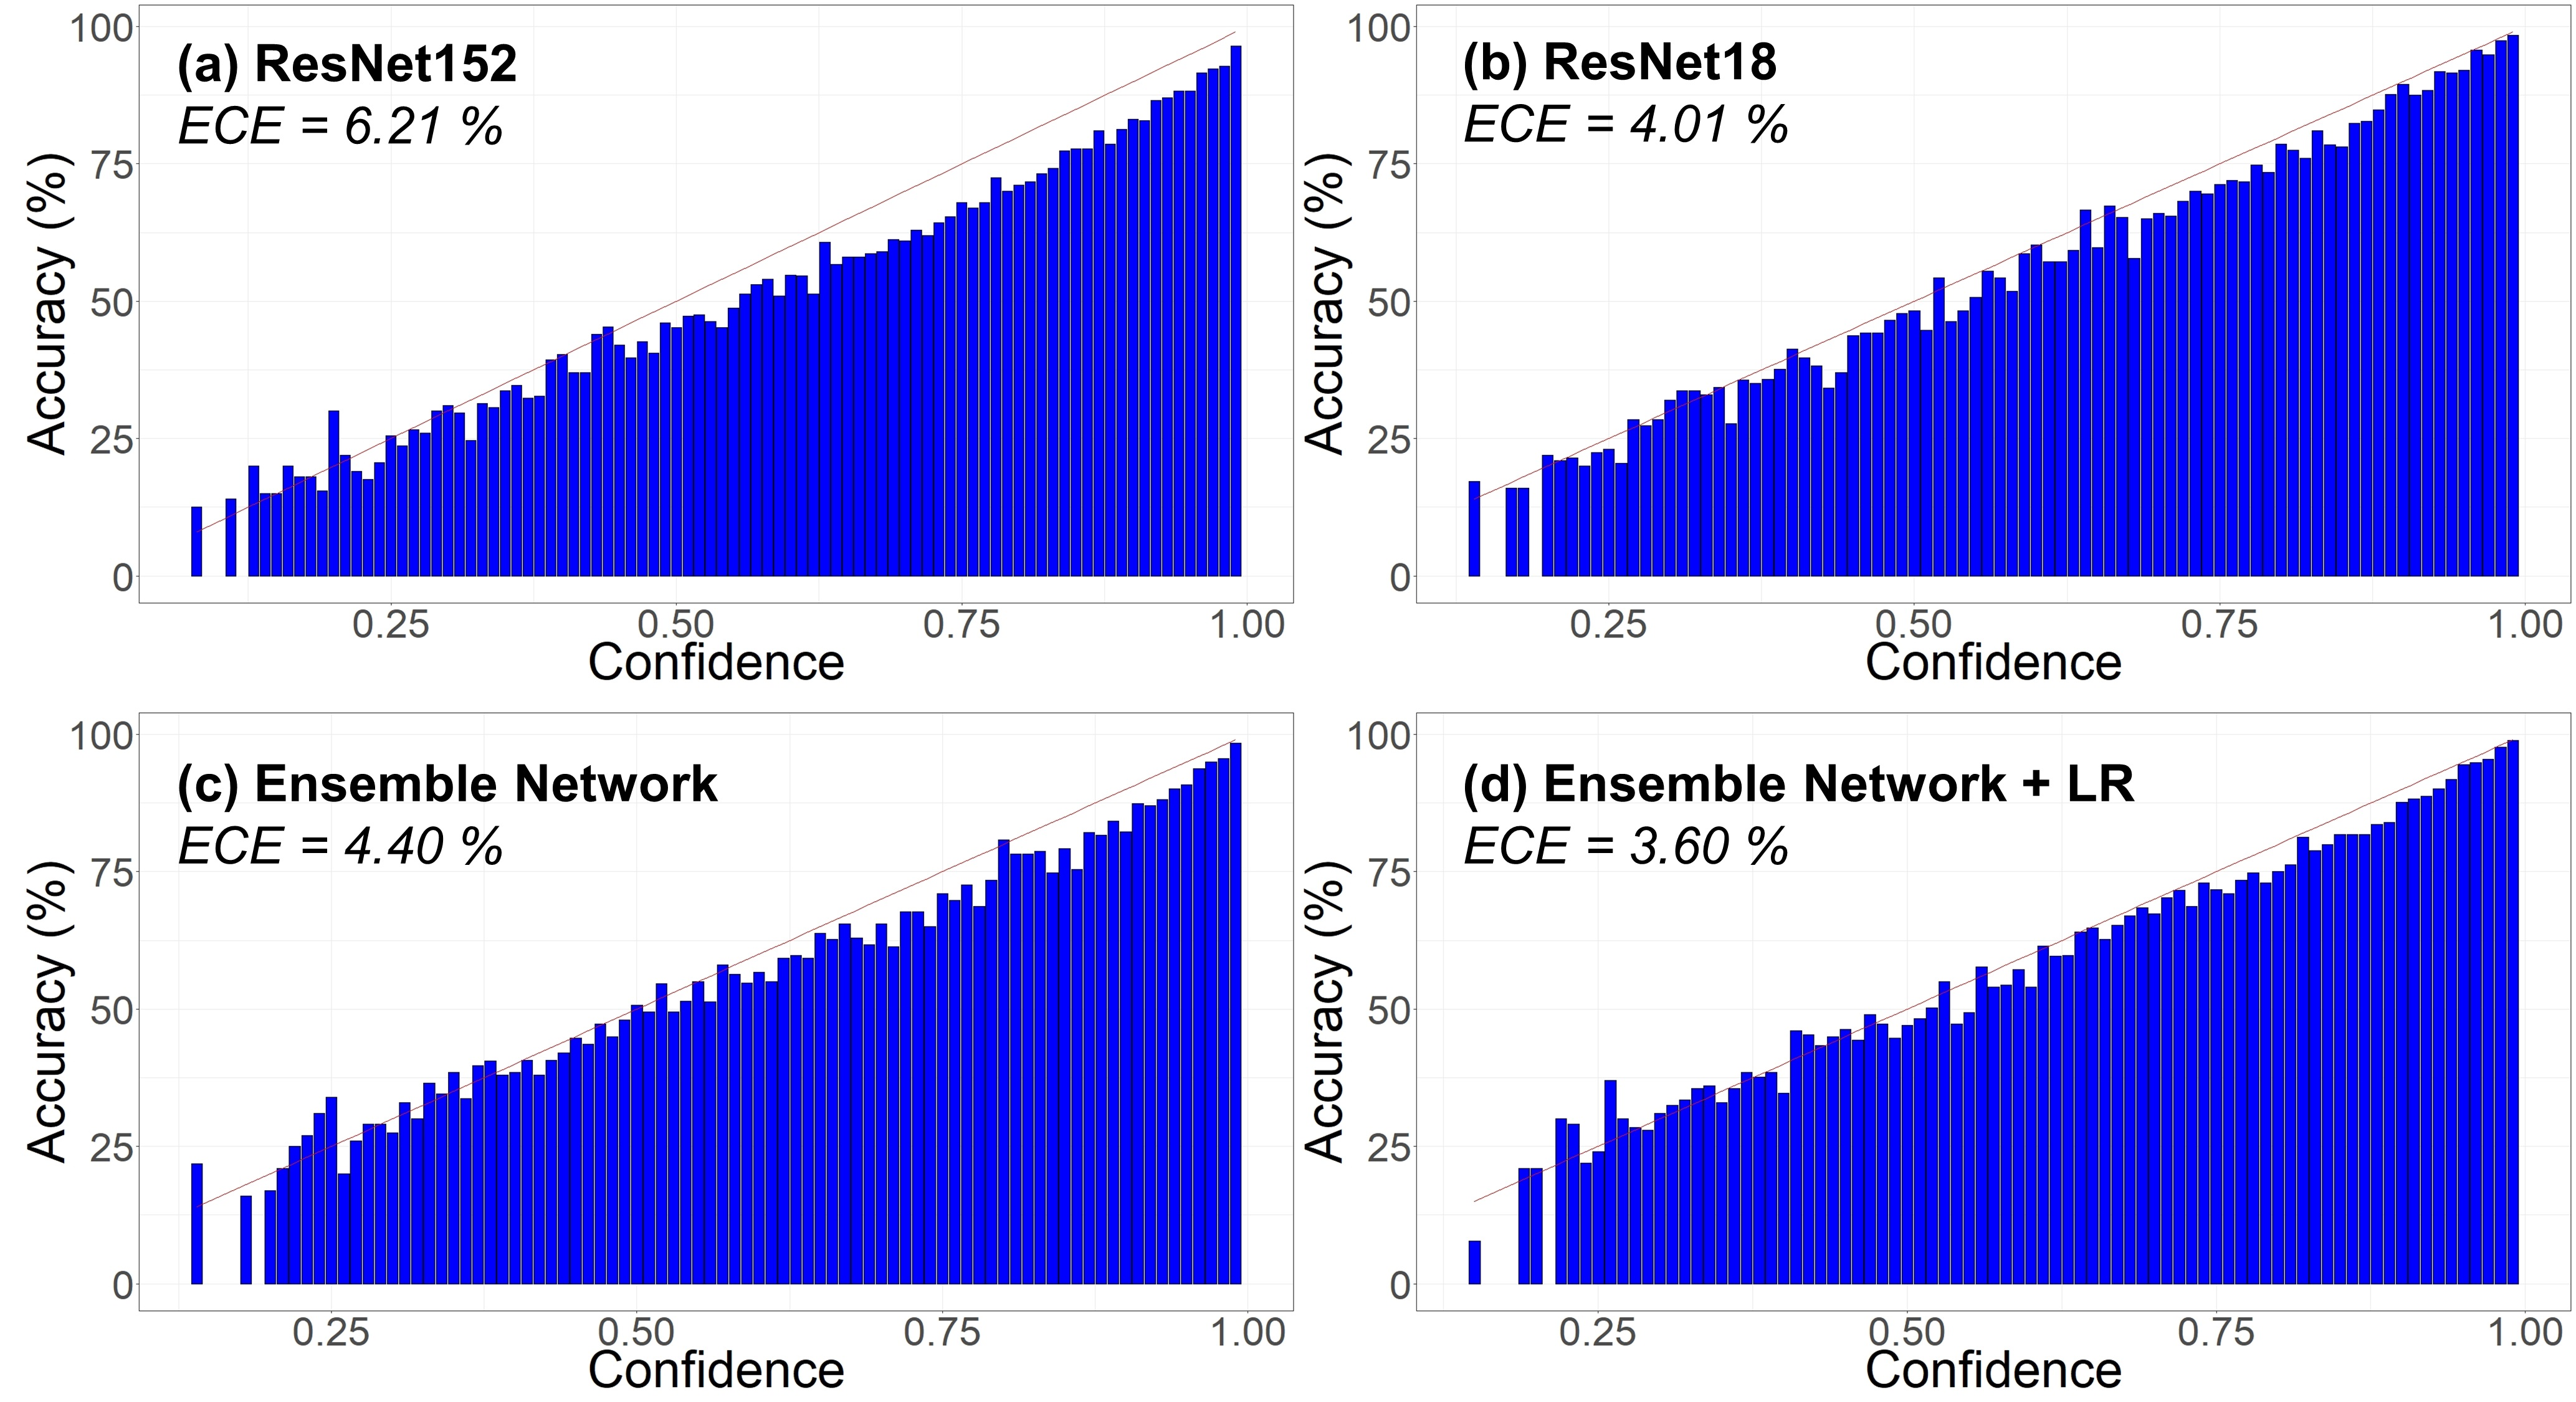
\includegraphics[width=\linewidth,keepaspectratio]{./3_chapitre1/Figure1.7}
		\caption[Reliability diagrams of the different networks]{Reliability diagrams of the different networks. The red curve corresponds to a perfect calibration (y = x). ECE = Estimated Calibration Error; ResNet152 = RestNet152 with patch size 224 × 224 and batch size 16; RestNet18 = RestNet18 with patch size \(224 \times 224\) and batch size 200; Ensemble Network = ensemble of the four ResNet18 with the four patch sizes (\(64 \times 64\), \(96 \times 96\), \(128 \times 128\) and \(224 \times 224\) pixels); Ensemble Network + LR = ensemble network with the logistic regression on the results of both the penultimate fully connected layer (fc256) and the softmax layer.}
	\label{figure1.7}
\end{center}
\end{figure}

The ResNet152 showed the highest ECE with 6.21 \%, while the best single ResNet18 (patch size 224 and batch size 200) achieved 4.01 \%. The ensemble network had an ECE of 4.40 \% without LR. The best score was achieved by the ensemble network with LR applied to the logits and the penultimate layer, which displayed an ECE of 3.60 \%.

\medskip

The results, recorded after the SGR algorithm was applied for selective classification on the best ensemble network with LR, are summarised in \autoref{table1.5}. A top-1 accuracy of 85.65 \% (risk = 14.35 \%) was achieved when covering 67.48 \% of the test set, and 91.30 \% accuracy (risk = 8.70 \%) could be obtained when classifying more than 50 \% of the data. Top-5 accuracy on the uncovered part of the data was consistently between 80 and 95 \%.

%%%%%%%%%%%%%%%%%%%%%%%%%%%%%%%%%%%%%%%%%%%%%%%%%%%%%%%%
%%% Table 1.5: Performances of logistic regression   %%%
%%%%%%%%%%%%%%%%%%%%%%%%%%%%%%%%%%%%%%%%%%%%%%%%%%%%%%%%
\begin{table}[htbp]
  \centering
  \normalsize
 % \raggedright
  \caption[Application of the Selection with Guaranteed Risk algorithm on the validation set for training and results on the test set]{Application of the Selection with Guaranteed Risk algorithm on the validation set for training and results on the test set. Top-5 uncovered = top-5 accuracy for the rejected part of the test set. All numbers are expressed in \%.}
  \label{table1.5}
    \begin{tabular}{@{}cccccc@{}}
        \toprule
        \textbf{Desired risk} & \textbf{Train-risk} & \textbf{Train-coverage} & \textbf{Test-risk} & \textbf{Test-coverage} & \textbf{Top-5 uncovered} \\ \midrule
        5.00                  & 4.25                & 33.98                   & 4.20               & 33.72                  & 94.16                    \\
        10.00                 & 9.15                & 52.12                   & 8.70               & 51.90                  & 92.71                    \\
        15.00                 & 14.11               & 67.59                   & 14.35              & 67.48                  & 91.06                    \\
        20.00                 & 19.09               & 80.47                   & 19.26              & 80.62                  & 88.16                    \\
        25.00                 & 24.08               & 92.97                   & 24.24              & 93.17                  & 81.75                    \\
        30.00                 & 27.30               & 100.00                  & 27.40              & 100.00                 & -                        \\ \bottomrule
    \end{tabular}
\end{table}

\subsubsection{Categories merging}\label{chapitre1_6.3.2}
Post-classification merging of the predicted classes, according to the taxonomic hierarchy, resulted in the consistent augmentation of performances (see \autoref{table1.6}). Gender grouping (level 2) led to a moderate increase of top-1 accuracy (75.91 \% vs 72.59 \% on the test set) and a small decrease in the total number of classes, from 61 to 56. Merging classes according to their major category (level 3) resulted in a gain of 11.88 points on the test set. The task was then reduced to discriminate between 15 classes, and results were then on par with the human accuracy tested on a 20 class task as recorded in Table 1 (72.88 macro-F1 and 84.29 micro-F1 on the test set versus 74.86 macro-F1 and 80.32 micro-F1 for host annotators on the human evaluation dataset).

%%%%%%%%%%%%%%%%%%%%%%%%%%%%%%%%%%%%%%%%%%%%%%%%%%%%%%%%
%%% Table 1.6: Performances of logistic regression   %%%
%%%%%%%%%%%%%%%%%%%%%%%%%%%%%%%%%%%%%%%%%%%%%%%%%%%%%%%%
\begin{table}[htbp]
  \centering
  \normalsize
 % \raggedright
  \caption[Results for coarse-to-fine categories merging according to taxonomic hierarchy]{Results for coarse-to-fine categories merging according to taxonomic hierarchy. Level 1 = original classes (61); level 2 = gender level (56); level 3 = major category level (15).}
  \label{table1.6}
  \begin{tabular}{*{2}{c}|*{3}{c}|*{3}{c}}
        \toprule
        \multicolumn{2}{c}{\textbf{}}               & \multicolumn{3}{c}{\textbf{Validation set}}                     & \multicolumn{3}{c}{\textbf{Test set}}                           \\ \midrule
        \textbf{Model} & \makecell{\textbf{Number} \\ \textbf{of classes}} & \textbf{Macro-F1} & \makecell{\textbf{Top-1} \\ \textbf{accuracy}} & \textbf{Micro-F1} & \textbf{Macro-F1} & \makecell{\textbf{Top-1} \\ \textbf{accuracy}} & \textbf{Micro-F1} \\
        \midrule
        Level 1        & 61                         & 63.74             & 72.69                   & 72.32             & 63.91             & 72.59                   & 72.20             \\
        Level 2        & 56                         & 64.86             & 75.98                   & 75.53             & 64.76             & 75.91                   & 75.63             \\
        Level 3        & 15                         & 71.75             & 84.40                   & 84.21             & 72.88             & 84.47                   & 84.29             \\ \bottomrule
    \end{tabular}
\end{table}

Level 3 merging offers an easy insight into the class-wise performance of the classification process (see \autoref{figure1.8}). Out of the 15 classes, three tended to be misclassified; “encrusting bryozoan” tended to be misclassified as “encrusting red macroalgae” (17 \%) and “sponge” (17 \%); “Hydroid” was often mistaken for “brown macroalgae” (19 \%) or “sludge, pavement, rubble, sand” (15 \%); and “sedentary worms” were most often misclassified as “encrusting red macroalgae” (16 \%) or “sludge, pavement, rubble, sand” (15 \%). Overall, four classes were responsible for most of the confusion: “brown macroalgae”, “encrusting red macroalgae”, “sponge”, and “sludge, pavement, rubble, sand”. On the other hand, seven classes tended to be well classified (> 80 \% accuracy): “encrusting red macroalgae” (92 \%), “gorgonian” (91 \%), “green macroalgae” (85 \%), “scleractinia” (87 \%), “sponge” (84 \%), “zoantharia” (89 \%) and “sludge, pavement, rubble, sand” (83 \%).

%%%%%%%%%%%%%%%%%%%%%%%%%%%%%%%%%%%%%%%%%%%%%%%%%%%%%%%%%%%%%%%%%%%%%%%%%%%%
%%% Figure 1.8: Confusion matrix of the output from the ensemble network %%%
%%%%%%%%%%%%%%%%%%%%%%%%%%%%%%%%%%%%%%%%%%%%%%%%%%%%%%%%%%%%%%%%%%%%%%%%%%%%
\begin{figure}[H]
	\begin{center}
	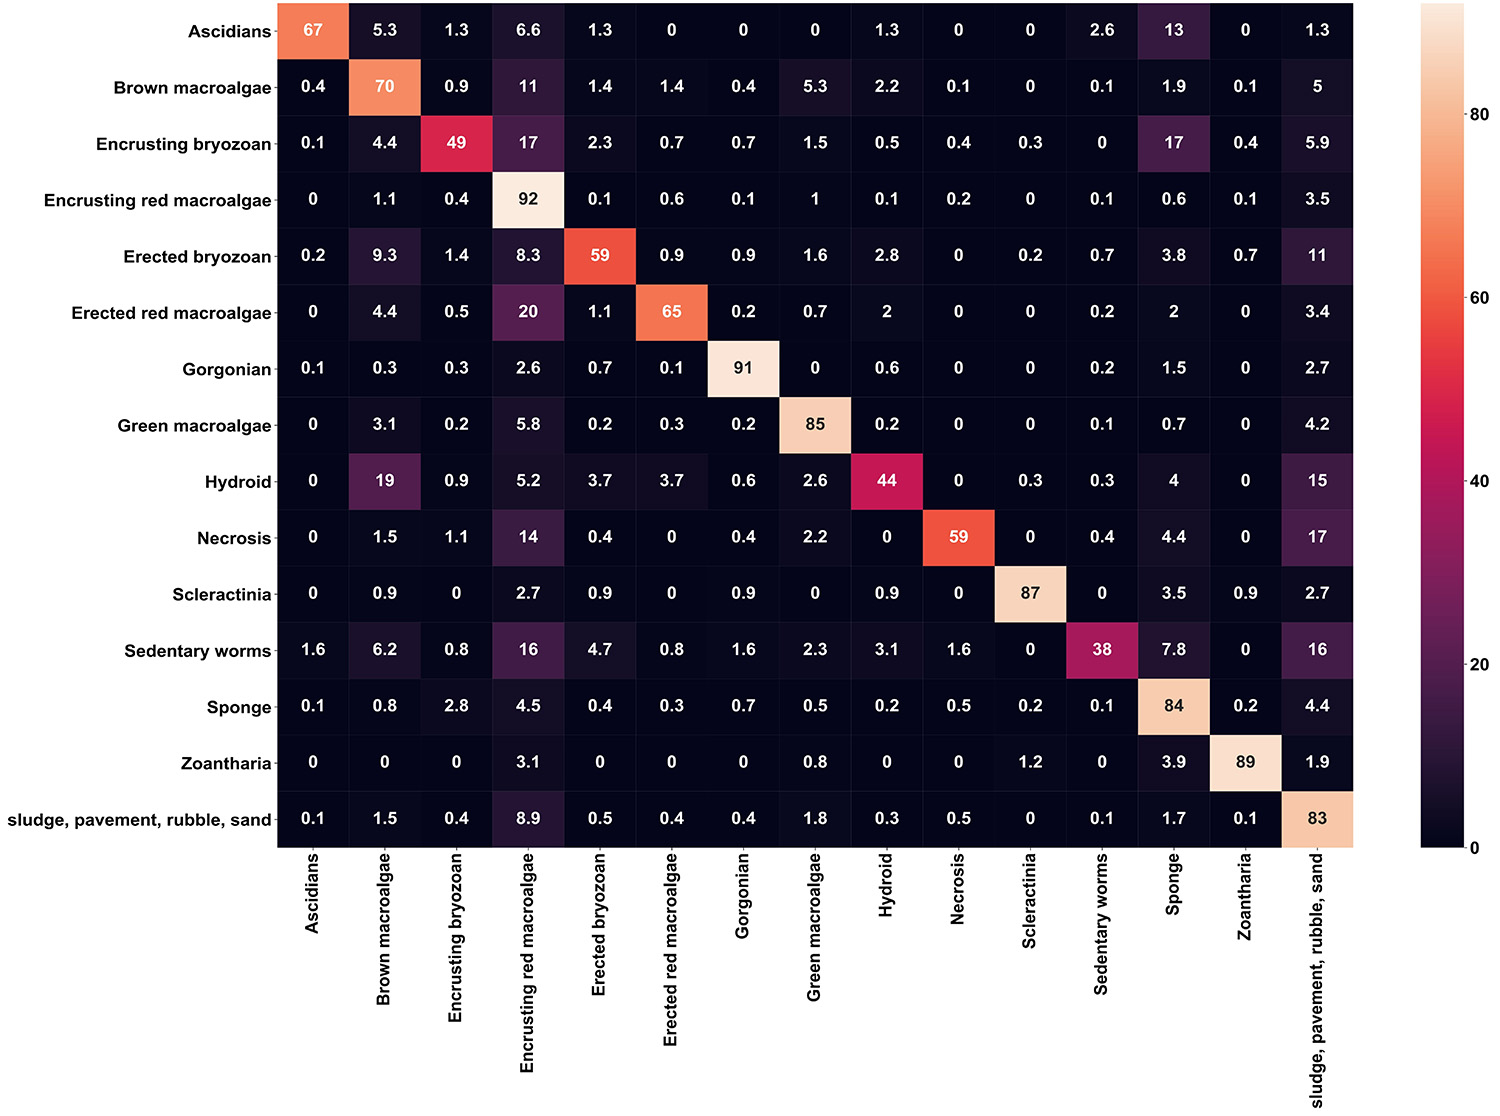
\includegraphics[width=\linewidth,keepaspectratio]{./3_chapitre1/Figure1.8}
		\caption[Confusion matrix of the output from the ensemble network with logistic regression on the test set]{Confusion matrix of the output from the ensemble network with logistic regression on the test set. The 61 original classes were merged to their major category (15 classes). Numbers represent ground truth repartition in predicted classes (\%).}
	\label{figure1.8}
\end{center}
\end{figure}

\newpage

\subsection{Ecological indicators prediction}\label{chapitre1_6.4}
Predicted sludge and bryozoans were correlated moderately well with the ground truth (see \autoref{figure1.9}; pearson correlation: 0.54 and 0.61, respectively), but predicted and observed major builders showed higher correlation (pearson correlation: 0.82).

%%%%%%%%%%%%%%%%%%%%%%%%%%%%%%%%%%%%%%%%%%%%%%%%%%%%%%%%
%%% Figure 1.9: sludge, bryozoans and major builders %%%
%%%%%%%%%%%%%%%%%%%%%%%%%%%%%%%%%%%%%%%%%%%%%%%%%%%%%%%%
\begin{figure}[H]
	\begin{center}
	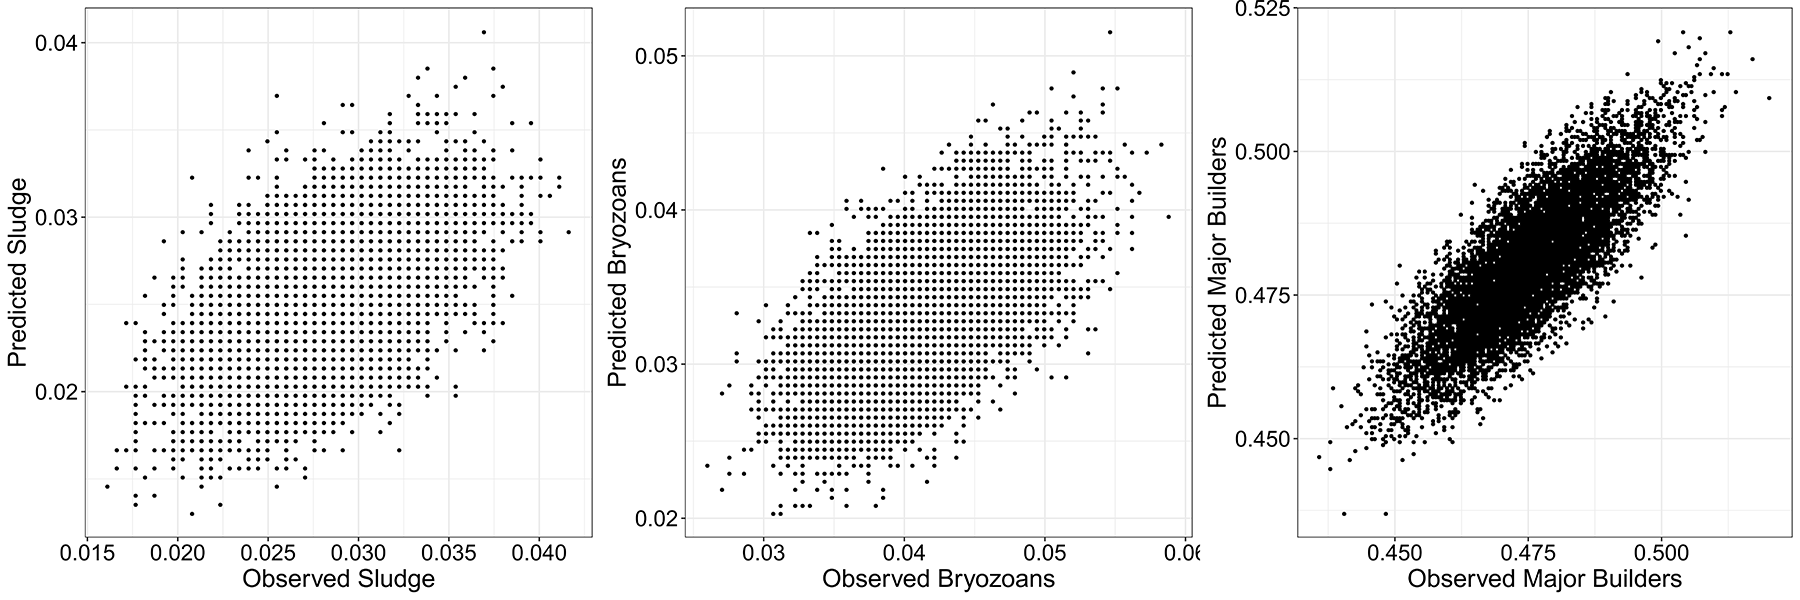
\includegraphics[width=\linewidth,keepaspectratio]{./3_chapitre1/Figure1.9}
		\caption[Predicted vs observed percentages of sludge, bryozoans and major builders]{Predicted vs observed percentages of sludge, bryozoans and major builders. Pearson correlations: Sludge = 0.54, Bryozoans = 0.61, Major builders = 0.82.}
	\label{figure1.9}
\end{center}
\end{figure}

Predicted CAI was moderately correlated with the ground truth (see \autoref{figure1.10}; pearson correlation: 0.61), but predicted and observed Shannon indices showed higher correlation (pearson correlation: 0.74).

%%%%%%%%%%%%%%%%%%%%%%%%%%%%%%%%%%%%%%%%%%%%%%%%%%%%%%%%%%%%%%%%%%%%%
%%% Figure 1.10: Coralligenous Assemblage Index and Shannon Index %%%
%%%%%%%%%%%%%%%%%%%%%%%%%%%%%%%%%%%%%%%%%%%%%%%%%%%%%%%%%%%%%%%%%%%%%
\begin{figure}[H]
	\begin{center}
	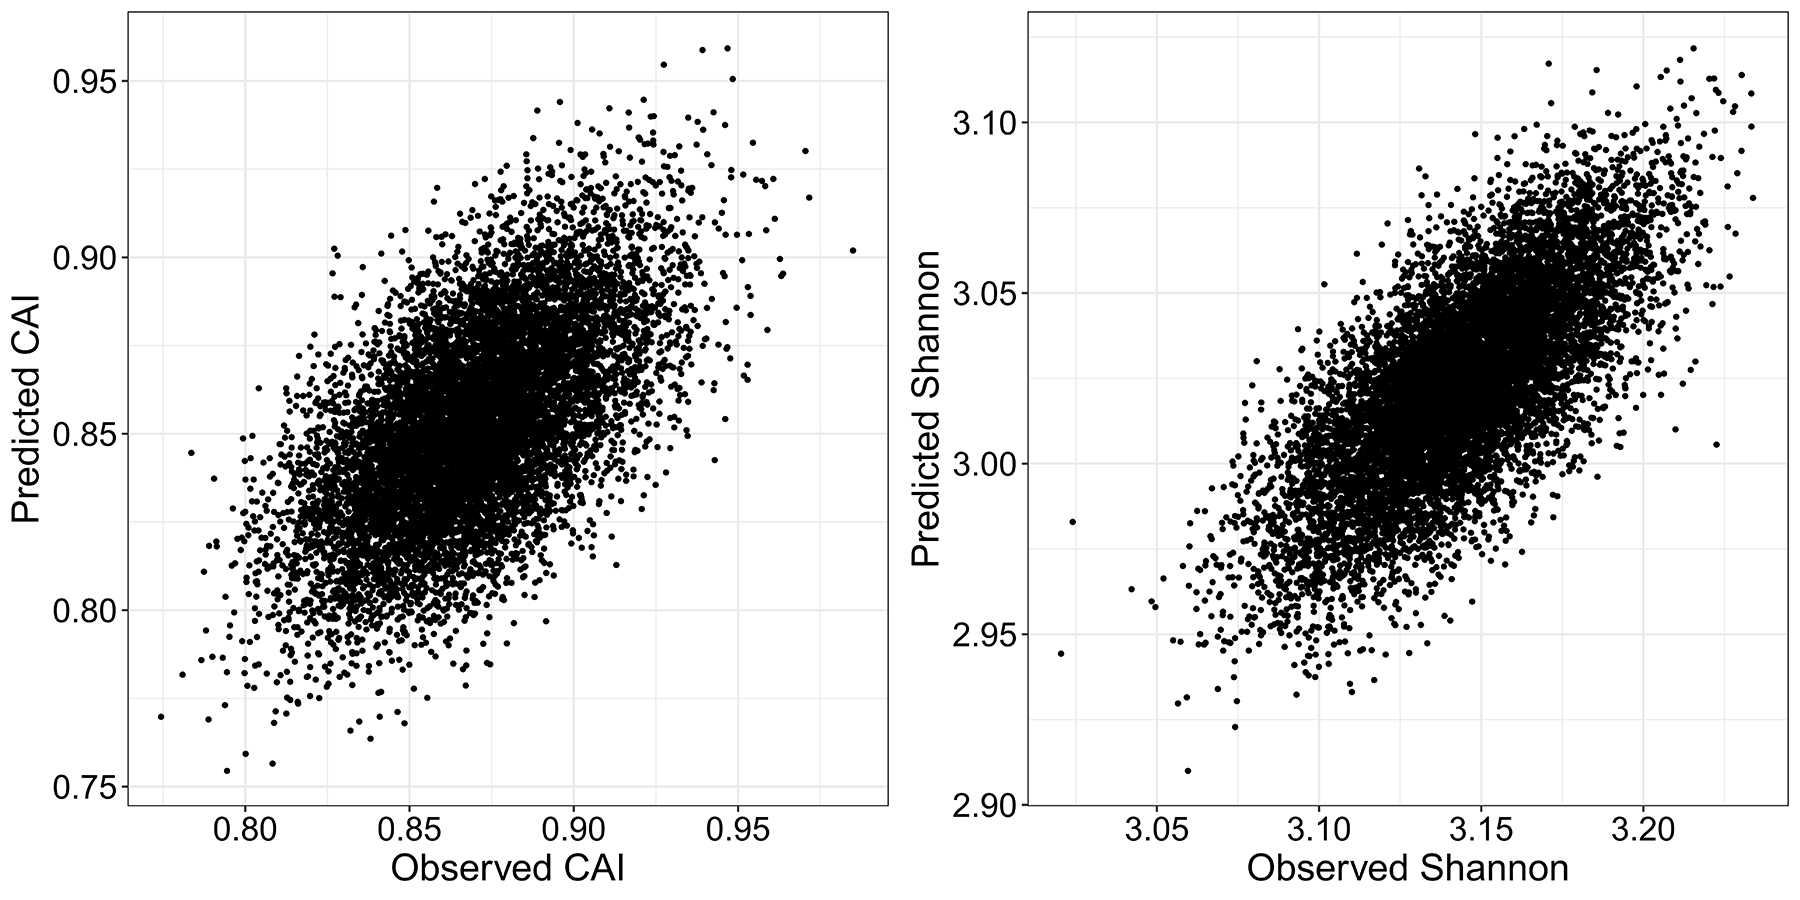
\includegraphics[width=0.7\linewidth,keepaspectratio]{./3_chapitre1/Figure1.10}
		\caption[Predicted vs observed Coralligenous Assemblage Index and Shannon Index]{Predicted vs observed Coralligenous Assemblage Index and Shannon Index. Pearson correlations: CAI = 0.61, Shannon Index = 0.74.}
	\label{figure1.10}
\end{center}
\end{figure}

\newpage

\section{Discussion}\label{chapitre1_7}

\subsection{Patch size influence}\label{chapitre1_7.1}
Although our dataset was large enough to train a CNN from scratch, it was limited to punctual annotations (at the pixel level) of photo quadrats, therefore it required patch-wise classification. The patch size was crucial (see \autoref{table1.2}), as it reflects a trade-off between local and contextual information. If the patch size is too small, it contains insufficient information and most probably fails to capture whole individuals; if it is too large, the context scrambles the signature of the central information, confusing the algorithm. The patch size \(64 \times 64\) pixels performed the worst out of all the metrics; the large differences between validation and test performances was indicative of its poor capacity for generalization. A patch size of \(224 \times 224\) gave the highest micro-F1 on the test set (65.94). This patch size included enough contextual noise to regularize overfitting, and it enabled better generalization. While the single RestNet18 based on the patch size \(224 \times 224\) obtained the best accuracy, our ensemble network, which was based on the four tested patch sizes and followed the feature extraction scheme of the local-SPP \citep{mahmood_coral_2016}, improved classification performances by 4.43 points (see \autoref{table1.3}). The biggest difference between our network and the original version of the local-SPP lies in the fact that we concatenated the four 512-dimension feature vectors, instead of the max-pooling layer, which enabled the information contributed by each patch size to be processed by the consecutive MLP without loss.

\subsection{Tuning the architecture}\label{chapitre1_7.2}
The training procedure of ResNet18, notably the batch size parameter, had a great impact on classification performance. This was indicated by the difference in micro-F1 values produced by a ResNet18 trained with batch size 128 (63.44; see \autoref{table1.3}) and a ResNet18 train with batch size 512 (65.54; see \autoref{table1.2}). These results provide a different perspective than the conclusions drawn by previous studies \citep{masters_revisiting_2018, mishkin_systematic_2016} where the use of small or even mini-batches enhanced performances. This could be explained by the high imbalance between classes and the fine-grained nature of the classification task. Larger batches may therefore be more representative of the intra-class variability which in turn allows the network to focus on inter-class variance. It will be asserted that our best ResNet18 (ResNet18---224; 65.94 micro-F1, see \autoref{table1.3}) easily outperformed deeper network architectures, whether trained from scratch with a smaller batch size (ResNet50---128; micro-F1 63.89), or pre-trained with fine-tuned weights (ResNet152---224; 60.09 micro-F1) according to standard procedures \citep{king_comparison_2018}. Our results support the findings of a recent study which advocated the use of carefully tailored training strategies and architecture enhancements for vastly improving performances, even with transfer learning \citep{he_bag_2019}. It remains to be said that further modifying the layers could further improve performances, for example altering the order of convolutions in residual blocks \citep{he_bag_2019} or widening the network \citep{zagoruyko_wide_2016}.

Training a LR on the penultimate and final layers of the ensemble network improved classification performances (72.20 vs 70.37 micro-F1, see \autoref{table1.4}). LRs derived from the results of the concatenation of the GAP or the first fully connected layer (fc512) greatly decreased performances on the validation set and led to a further decrease in performance on the test set, indicating that the LR massively overfitted the training set. It is widely known that using a CNN in combination with other machine learning algorithms can improve classification accuracy \citep{donahue_decaf:_2014, gao_combining_2017, huang_densely_2017, li_visual_2016}, but additionally applying them to the logits of a neural network is further beneficial to the use of a selective classification framework, LR is a linear classifier that uses negative log-likelihood (NLL) as a loss function for a multiclass problem. When feeding the logits taken from the last layer of the ensemble network into a softmax, it performs linear scaling to optimise the NLL in a similar way that temperature scaling can be used for network calibration \citep{guo_calibration_2017}. This explains why applying LR to the last two layers of the ensemble network improved calibration (ECE = 3.60 \%) while simultaneously improving performance. The fact that ResNet152 was the worst calibrated (ECE = 6.21 \%) is coherent with previous studies’ findings, which noted that the depth and width of the network negatively impact calibration \citep{guo_calibration_2017}. This also applies to the ensemble network (ECE = 4.40 \%), which was slightly deeper and considerably wider than a single ResNet18---224 (ECE = 4.01 \%).

\subsection{Post-processing}\label{chapitre1_7.3}
Selective classification requires well-calibrated networks because the reliability of the output is assessed in order to decide whether or not to reject the prediction. The SGR algorithm provides accurate thresholds which allow the user to filter predictions which fit with the required level of error \citep{geifman_selective_2017}. Top-5 accuracy was consistently above 80 \% on the rejected part on the test set, regardless of desired risk specified for input into the SGR algorithm. Said top-5 accuracy could then be used to create a tool to enable an expert to quickly annotate the rejected data. By establishing a trade-off between accuracy and time-effectiveness, this simple method could be useful for mitigating the limited accuracy of human annotation (which in turn affects performance in the classification task), and is appropriate considering the fine-grained nature of the classification task.

Further customising the network, we merged the output classes by gender and major categories. While merging gender classes (61 to 54 classes) improved performance by one to three points (level 2, see \autoref{table1.6}), major category merging (61 to 15 classes) improved performance by eight to twelve points, depending on the metrics considered (level 3, see \autoref{table1.6}). These results indicated that the error observed in level 1 classification makes biological sense, as class confusions are for the most part taxonomically coherent. Major category merging enabled us to easily detect the repartition of the error (see \autoref{figure1.8}), wherein three categories were ill-predicted (“Encrusting bryozoan”, “Hydroid” and “Sedentary worms”), and a further four categories induced a great deal of confusion (“Brown macroalgae”, “Encrusting red macroalgae”, “Sponge”, and “Sludge, pavement, rubble, sand”). This can be explained by the imbalance of the classes in the dataset: the network misses examples for poorly represented classes and tends to misclassify those as one of the four predominant classes that are visible in most of the patches, such as “Encrusting red macroalgae”.. This also explains why macro metrics, which place equal weight on each class, performed consistently worse than micro metrics. This disparity of performance could certainly be ameliorated by an addition of instances, since the availability of data regarding class has been shown to directly influence performance \citep{zhou_learning_2014}. The confusion experienced by the network may be explained by the nature of the habitat to a certain extent. For example, it makes sense that the major category “sludge, pavement, rubble, sand” generated a great deal of noise, since lots of individuals in the benthos were partially covered by sediment particles.

Finally, it should be noted that, by merging the outputs to 15 major categories, the accuracy scores achieved when considering the relative abundance of classes in the dataset (i.e. micro metrics) outperformed the human accuracy observed on a similar problem conducted on 20 coral reef classes at the gender level \citep{beijbom_towards_2015}. If no conclusion can be directly drawn from this observation, it nevertheless represents a significant achievement given the high level of similarity between coral and coralligenous habitats \citep{bianchi_biocostruzione_2001}, and the fact that some major categories defined here were included in the task presented by Beijbom et al. The annotator accuracy also gives a general indication of the noisiness of the annotated dataset used for training and testing. In this study, the annotations were performed only once by a single annotator, which means that our dataset includes errors learned by our networks. This explains part of the irreducible error made by our networks, as previous studies have shown how this impedes network efficiency \citep{mishkin_systematic_2016}. However, results per class showed that scarcity of data, and confusion between similar species were the greatest source of error. 

\subsection{On the use of CNNs in a large scale monotoring of coralligenous reefs}\label{chapitre1_7.4}
Monitoring coralligenous reefs involves long, physically demanding dives at great depths below sea level (often 40---80 m deep), and many hours spent on the task of manually identifying species in photo quadrats \citep{deter_rapid_2012}. The use of well-trained CNNs (particularly those which operate within a selective classification framework) can greatly aid this process; it makes the automatic annotation of vast quantities of data possible, while ensuring a guaranteed accuracy. At the level of detail “major category” (level 3, see \autoref{table1.6}), which can suffice for a quick evaluation of the diversity, our CNN performance even exceeded the human accuracy measured on a similar dataset when considering the relative abundance of classes in the dataset (i.e. micro metrics; see Table 1). In order to further refine the classification and obtain a more detailed assessment that includes rare or invasive species, this problem could be addressed by the use of few-shot or even zero-shot learning \citep{liu_generalized_2018}.

The predicted percentages of major builders was fairly accurate, with a high correlation between observed and predicted values (pearson correlation: 0.82; see \autoref{figure1.9}). The predictions of sludge and bryozoans on the other hand were altogether less accurate, with a weaker correlation between observations and predictions (pearson correlation: 0.54 and 0.61, respectively). The various substrates were divided into four different categories: “sludge”, “pavement”, “rubble”, and “sand”. Given the similarity of the substrates, they are subject to the arbitrary interpretation of the expert and are therefore fairly likely to contain annotator errors. Consequently, 11 \% of “sludge” instances were classified as “sand”, and a further 2 \% was classified as “rubble”. What is more, “sludge” instances often corresponded to very small patches of sludge atop more easily recognizable classes, which confused the algorithm on a number of occasions. For example, 7 \% of sludge instances were confused with Mesophyllum alternans, and a further 5 \% with encrusting \textit{Peyssonnelia sp.} – these are two different encrusting, red macroalgae. While the classification of “encrusting red macroalgae” at level 3 clustering was highly accurate (92 \% , see \autoref{figure1.8}), it should be noted that “encrusting bryozoan” and “erected bryozoan” were sometimes confused with “encrusting red macroalgae”, “sponge” and substrate. All of these factors affected CAI predictions (pearson correlation: 0.61; see Figure 10) which are based on proportions of major builders, bryozoans and sludge. However, assessment of biodiversity was more accurate; the correlation between predicted and observed Shannon index values was 0.74. These results suggest that our method can be used to quickly assess the diversity of multiple sites within a large-scale monitoring network.

\section{Conclusions}\label{chapitre1_8}
\noindent Considering the high complexity and heterogeneity of coralligenous reefs, the results we achieved on this 61-class task attained so high a level of refinement of prediction as to constitute a real advance in automated benthic species recognition. The use of multi-scale analysis for processing various levels of local information proved very effective for addressing the task at hand, and the use of a logistic regression on deeply learned features successfully enhanced our results, producing well-calibrated predictions. In sum, this project culminated in the development of a semi-automated, species recognition tool for analysing photo quadrats of coralligenous reefs which can be adjusted to match the required levels of accuracy and detail, at the cost of a decrease in the classification rate. To conclude, this study represents a milestone for the development of an effective, automated assessment protocol for measuring the ecological status of coralligenous reefs. However, deep learning knows very fast improvements, and our methodology could benefit from the latest findings in order to improve some of the components of our pipeline. Future work made in this field would also benefit from a combination of deep learning approaches and photogrammetry, as combining biodiversity assessment and 3D structural indicators enables the exploration of the links between structural complexity and ecosystem functioning indices. 

\newpage